\documentclass[twoside]{book}

% Packages required by doxygen
\usepackage{fixltx2e}
\usepackage{calc}
\usepackage{doxygen}
\usepackage[export]{adjustbox} % also loads graphicx
\usepackage{graphicx}
\usepackage[utf8]{inputenc}
\usepackage{makeidx}
\usepackage{multicol}
\usepackage{multirow}
\PassOptionsToPackage{warn}{textcomp}
\usepackage{textcomp}
\usepackage[nointegrals]{wasysym}
\usepackage[table]{xcolor}

% Font selection
\usepackage[T1]{fontenc}
\usepackage[scaled=.90]{helvet}
\usepackage{courier}
\usepackage{amssymb}
\usepackage{sectsty}
\renewcommand{\familydefault}{\sfdefault}
\allsectionsfont{%
  \fontseries{bc}\selectfont%
  \color{darkgray}%
}
\renewcommand{\DoxyLabelFont}{%
  \fontseries{bc}\selectfont%
  \color{darkgray}%
}
\newcommand{\+}{\discretionary{\mbox{\scriptsize$\hookleftarrow$}}{}{}}

% Page & text layout
\usepackage{geometry}
\geometry{%
  a4paper,%
  top=2.5cm,%
  bottom=2.5cm,%
  left=2.5cm,%
  right=2.5cm%
}
\tolerance=750
\hfuzz=15pt
\hbadness=750
\setlength{\emergencystretch}{15pt}
\setlength{\parindent}{0cm}
\setlength{\parskip}{3ex plus 2ex minus 2ex}
\makeatletter
\renewcommand{\paragraph}{%
  \@startsection{paragraph}{4}{0ex}{-1.0ex}{1.0ex}{%
    \normalfont\normalsize\bfseries\SS@parafont%
  }%
}
\renewcommand{\subparagraph}{%
  \@startsection{subparagraph}{5}{0ex}{-1.0ex}{1.0ex}{%
    \normalfont\normalsize\bfseries\SS@subparafont%
  }%
}
\makeatother

% Headers & footers
\usepackage{fancyhdr}
\pagestyle{fancyplain}
\fancyhead[LE]{\fancyplain{}{\bfseries\thepage}}
\fancyhead[CE]{\fancyplain{}{}}
\fancyhead[RE]{\fancyplain{}{\bfseries\leftmark}}
\fancyhead[LO]{\fancyplain{}{\bfseries\rightmark}}
\fancyhead[CO]{\fancyplain{}{}}
\fancyhead[RO]{\fancyplain{}{\bfseries\thepage}}
\fancyfoot[LE]{\fancyplain{}{}}
\fancyfoot[CE]{\fancyplain{}{}}
\fancyfoot[RE]{\fancyplain{}{\bfseries\scriptsize Generated by Doxygen }}
\fancyfoot[LO]{\fancyplain{}{\bfseries\scriptsize Generated by Doxygen }}
\fancyfoot[CO]{\fancyplain{}{}}
\fancyfoot[RO]{\fancyplain{}{}}
\renewcommand{\footrulewidth}{0.4pt}
\renewcommand{\chaptermark}[1]{%
  \markboth{#1}{}%
}
\renewcommand{\sectionmark}[1]{%
  \markright{\thesection\ #1}%
}

% Indices & bibliography
\usepackage{natbib}
\usepackage[titles]{tocloft}
\setcounter{tocdepth}{3}
\setcounter{secnumdepth}{5}
\makeindex

% Hyperlinks (required, but should be loaded last)
\usepackage{ifpdf}
\ifpdf
  \usepackage[pdftex,pagebackref=true]{hyperref}
\else
  \usepackage[ps2pdf,pagebackref=true]{hyperref}
\fi
\hypersetup{%
  colorlinks=true,%
  linkcolor=blue,%
  citecolor=blue,%
  unicode%
}

% Custom commands
\newcommand{\clearemptydoublepage}{%
  \newpage{\pagestyle{empty}\cleardoublepage}%
}

\usepackage{caption}
\captionsetup{labelsep=space,justification=centering,font={bf},singlelinecheck=off,skip=4pt,position=top}

%===== C O N T E N T S =====

\begin{document}

% Titlepage & ToC
\hypersetup{pageanchor=false,
             bookmarksnumbered=true,
             pdfencoding=unicode
            }
\pagenumbering{alph}
\begin{titlepage}
\vspace*{7cm}
\begin{center}%
{\Large Q\+Mesh }\\
\vspace*{1cm}
{\large Generated by Doxygen 1.8.13}\\
\end{center}
\end{titlepage}
\clearemptydoublepage
\pagenumbering{roman}
\tableofcontents
\clearemptydoublepage
\pagenumbering{arabic}
\hypersetup{pageanchor=true}

%--- Begin generated contents ---
\chapter{Q\+Mesh Mbed Studio Project}
\label{md_README}
\Hypertarget{md_README}
Q\+Mesh is a synchronized flooded mesh network designed to stream at a low data rate. While the data rate is slow, it should suffice for e.\+g. Codec2 voice data. This initial Proof-\/of-\/\+Concept leverages the A\+RM Mbed framework, the S\+T\+M32 Nucleo series of S\+T\+M32 development boards, and Arduino and Mbed shields.

\subsection*{Mitigating the collision/broadcast storm problem}

In a synchronized, flooded mesh, all nodes retransmit at roughly the same time, creating collisions. Lo\+Ra, a form of Chirp Spread Spectrum (C\+SS), possesses several unique properties that can allow for successful receipt of one packet in the midst of one or more collisions. First, spread spectrum modulations (C\+SS as well as D\+S\+SS and F\+H\+SS) spread signal energy such that concurrent transmissions are less likely to overlap and thus interfere. Second, Semtech\textquotesingle{}s Lo\+Ra chipsets allow for a per-\/data-\/symbol frequency hopping that can further spread concurrent transmissions from each other. This F\+H\+SS can also be combined with a form of slotted A\+L\+O\+HA to greatly reduce the probability that packets will collide at all. Third, Lo\+Ra is highly resistant to frequency error. Deliberately adding frequency error can spread out concurrent transmissions so that they do not interfere with each other.

\subsection*{Licensing.}

Q\+Mesh is licensed under the G\+NU G\+PL License v3; however, a commercial license is also available for entities who do not want to release their source code changes. Please contact Dan Fay at \href{mailto:daniel.fay@gmail.com}{\tt daniel.\+fay@gmail.\+com} for more information about this. 
\chapter{Namespace Index}
\section{Namespace List}
Here is a list of all documented namespaces with brief descriptions\+:\begin{DoxyCompactList}
\item\contentsline{section}{\hyperlink{namespacembed__settings}{mbed\+\_\+settings} }{\pageref{namespacembed__settings}}{}
\end{DoxyCompactList}

\chapter{Hierarchical Index}
\doxysection{Class Hierarchy}
This inheritance list is sorted roughly, but not completely, alphabetically\+:\begin{DoxyCompactList}
\item \contentsline{section}{Frame\+::crc16\+\_\+t}{\pageref{unionFrame_1_1crc16__t}}{}
\item \contentsline{section}{D\+R\+A818}{\pageref{classDRA818}}{}
\item \contentsline{section}{F\+EC}{\pageref{classFEC}}{}
\begin{DoxyCompactList}
\item \contentsline{section}{F\+E\+C\+Interleave}{\pageref{classFECInterleave}}{}
\begin{DoxyCompactList}
\item \contentsline{section}{F\+E\+C\+Conv}{\pageref{classFECConv}}{}
\begin{DoxyCompactList}
\item \contentsline{section}{F\+E\+C\+R\+SV}{\pageref{classFECRSV}}{}
\end{DoxyCompactList}
\end{DoxyCompactList}
\end{DoxyCompactList}
\item \contentsline{section}{Frame}{\pageref{classFrame}}{}
\item \contentsline{section}{Indicator\+L\+ED}{\pageref{classIndicatorLED}}{}
\item \contentsline{section}{J\+S\+O\+N\+Serial}{\pageref{classJSONSerial}}{}
\item \contentsline{section}{Nucleo144\+L\+E\+Ds}{\pageref{classNucleo144LEDs}}{}
\item \contentsline{section}{nv\+\_\+settings\+\_\+t}{\pageref{structnv__settings__t}}{}
\item \contentsline{section}{Push\+Button}{\pageref{classPushButton}}{}
\item \contentsline{section}{Radio\+Event}{\pageref{classRadioEvent}}{}
\item \contentsline{section}{Radio\+Timing}{\pageref{classRadioTiming}}{}
\end{DoxyCompactList}

\chapter{Class Index}
\section{Class List}
Here are the classes, structs, unions and interfaces with brief descriptions\+:\begin{DoxyCompactList}
\item\contentsline{section}{\hyperlink{unionFrame_1_1crc16__t}{Frame\+::crc16\+\_\+t} }{\pageref{unionFrame_1_1crc16__t}}{}
\item\contentsline{section}{\hyperlink{classFEC}{F\+EC} }{\pageref{classFEC}}{}
\item\contentsline{section}{\hyperlink{classFECConv}{F\+E\+C\+Conv} }{\pageref{classFECConv}}{}
\item\contentsline{section}{\hyperlink{classFECInterleave}{F\+E\+C\+Interleave} }{\pageref{classFECInterleave}}{}
\item\contentsline{section}{\hyperlink{classFECPolar}{F\+E\+C\+Polar} }{\pageref{classFECPolar}}{}
\item\contentsline{section}{\hyperlink{classFECRSV}{F\+E\+C\+R\+SV} }{\pageref{classFECRSV}}{}
\item\contentsline{section}{\hyperlink{classFrame}{Frame} }{\pageref{classFrame}}{}
\item\contentsline{section}{\hyperlink{classIndicatorLED}{Indicator\+L\+ED} }{\pageref{classIndicatorLED}}{}
\item\contentsline{section}{\hyperlink{classJSONSerial}{J\+S\+O\+N\+Serial} }{\pageref{classJSONSerial}}{}
\item\contentsline{section}{\hyperlink{structnv__settings__t}{nv\+\_\+settings\+\_\+t} }{\pageref{structnv__settings__t}}{}
\item\contentsline{section}{\hyperlink{classPushButton}{Push\+Button} }{\pageref{classPushButton}}{}
\item\contentsline{section}{\hyperlink{classRadioEvent}{Radio\+Event} }{\pageref{classRadioEvent}}{}
\item\contentsline{section}{\hyperlink{classRadioFrequency}{Radio\+Frequency} }{\pageref{classRadioFrequency}}{}
\item\contentsline{section}{\hyperlink{classRadioTiming}{Radio\+Timing} }{\pageref{classRadioTiming}}{}
\end{DoxyCompactList}

\chapter{Namespace Documentation}
\hypertarget{namespacembed__settings}{}\section{mbed\+\_\+settings Namespace Reference}
\label{namespacembed__settings}\index{mbed\+\_\+settings@{mbed\+\_\+settings}}


\subsection{Detailed Description}
\begin{DoxyVerb}mbed SDK
Copyright (c) 2016 ARM Limited

Licensed under the Apache License, Version 2.0 (the "License");
you may not use this file except in compliance with the License.
You may obtain a copy of the License at

http://www.apache.org/licenses/LICENSE-2.0

Unless required by applicable law or agreed to in writing, software
distributed under the License is distributed on an "AS IS" BASIS,
WITHOUT WARRANTIES OR CONDITIONS OF ANY KIND, either express or implied.
See the License for the specific language governing permissions and
limitations under the License.
\end{DoxyVerb}
 
\chapter{Class Documentation}
\hypertarget{unionFrame_1_1crc16__t}{}\section{Frame\+:\+:crc16\+\_\+t Union Reference}
\label{unionFrame_1_1crc16__t}\index{Frame\+::crc16\+\_\+t@{Frame\+::crc16\+\_\+t}}
\subsection*{Public Attributes}
\begin{DoxyCompactItemize}
\item 
\mbox{\Hypertarget{unionFrame_1_1crc16__t_a230eea3ba9cb081e8e6d62bbf2a3f98f}\label{unionFrame_1_1crc16__t_a230eea3ba9cb081e8e6d62bbf2a3f98f}} 
uint16\+\_\+t {\bfseries crc}
\item 
\mbox{\Hypertarget{unionFrame_1_1crc16__t_ae785c01c5ae636921bbfc063c17d571f}\label{unionFrame_1_1crc16__t_ae785c01c5ae636921bbfc063c17d571f}} 
uint8\+\_\+t {\bfseries crc\+\_\+bytes} \mbox{[}2\mbox{]}
\end{DoxyCompactItemize}


The documentation for this union was generated from the following file\+:\begin{DoxyCompactItemize}
\item 
inc/serial\+\_\+data.\+hpp\end{DoxyCompactItemize}

\hypertarget{classFEC}{}\doxysection{F\+EC Class Reference}
\label{classFEC}\index{FEC@{FEC}}


{\ttfamily \#include $<$fec.\+hpp$>$}



Inheritance diagram for F\+EC\+:\nopagebreak
\begin{figure}[H]
\begin{center}
\leavevmode
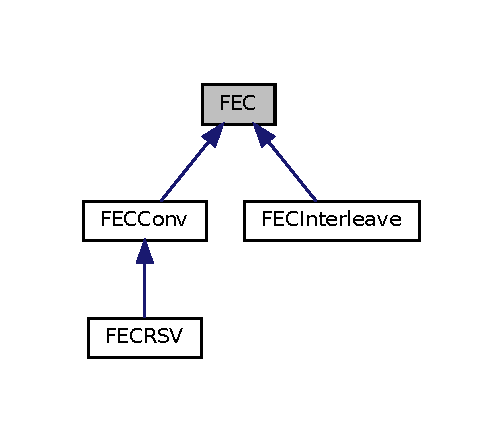
\includegraphics[width=165pt]{classFEC__inherit__graph}
\end{center}
\end{figure}
\doxysubsection*{Public Member Functions}
\begin{DoxyCompactItemize}
\item 
\mbox{\Hypertarget{classFEC_a0f673c71e8de7160c45439c335dd9de8}\label{classFEC_a0f673c71e8de7160c45439c335dd9de8}} 
\mbox{\hyperlink{classFEC_a0f673c71e8de7160c45439c335dd9de8}{F\+EC}} (const int32\+\_\+t my\+\_\+msg\+\_\+len)
\begin{DoxyCompactList}\small\item\em Constructor. \end{DoxyCompactList}\item 
\mbox{\Hypertarget{classFEC_afd2e56aa5a55ba34dc52e01a221c1350}\label{classFEC_afd2e56aa5a55ba34dc52e01a221c1350}} 
string \mbox{\hyperlink{classFEC_afd2e56aa5a55ba34dc52e01a221c1350}{get\+Name}} (void)
\begin{DoxyCompactList}\small\item\em Gets the name of the \mbox{\hyperlink{classFEC}{F\+EC}}. \end{DoxyCompactList}\item 
virtual int32\+\_\+t \mbox{\hyperlink{classFEC_adbb1c8a7c0b252bad75aab2bad731330}{encode}} (const vector$<$ uint8\+\_\+t $>$ \&msg, vector$<$ uint8\+\_\+t $>$ \&enc\+\_\+msg)
\item 
virtual int32\+\_\+t \mbox{\hyperlink{classFEC_a04b574b82bebfb6388ee2274e17f0222}{decode}} (const vector$<$ uint8\+\_\+t $>$ \&enc\+\_\+msg, vector$<$ uint8\+\_\+t $>$ \&dec\+\_\+msg)
\item 
\mbox{\Hypertarget{classFEC_acf5701c0025cdd86df8cc0a3dd6a7460}\label{classFEC_acf5701c0025cdd86df8cc0a3dd6a7460}} 
void {\bfseries benchmark} (const size\+\_\+t num\+\_\+iters)
\end{DoxyCompactItemize}
\doxysubsection*{Public Attributes}
\begin{DoxyCompactItemize}
\item 
\mbox{\Hypertarget{classFEC_a396a1f4d4c2594d0da67934771d75e2e}\label{classFEC_a396a1f4d4c2594d0da67934771d75e2e}} 
int {\bfseries enc\+\_\+size}
\end{DoxyCompactItemize}
\doxysubsection*{Protected Attributes}
\begin{DoxyCompactItemize}
\item 
\mbox{\Hypertarget{classFEC_abb6d143bc35d00ea0d302b1f70af9851}\label{classFEC_abb6d143bc35d00ea0d302b1f70af9851}} 
string {\bfseries name}
\item 
\mbox{\Hypertarget{classFEC_a03c5ef31ae69001bf8818f8d05683700}\label{classFEC_a03c5ef31ae69001bf8818f8d05683700}} 
int {\bfseries msg\+\_\+len}
\end{DoxyCompactItemize}


\doxysubsection{Detailed Description}
Base class for Forward Error Correction. Provides some generically-\/useful functions, like interleaving, but otherwise just functions as a dummy \mbox{\hyperlink{classFEC}{F\+EC}} class. 

\doxysubsection{Member Function Documentation}
\mbox{\Hypertarget{classFEC_a04b574b82bebfb6388ee2274e17f0222}\label{classFEC_a04b574b82bebfb6388ee2274e17f0222}} 
\index{FEC@{FEC}!decode@{decode}}
\index{decode@{decode}!FEC@{FEC}}
\doxysubsubsection{\texorpdfstring{decode()}{decode()}}
{\footnotesize\ttfamily virtual int32\+\_\+t F\+E\+C\+::decode (\begin{DoxyParamCaption}\item[{const vector$<$ uint8\+\_\+t $>$ \&}]{enc\+\_\+msg,  }\item[{vector$<$ uint8\+\_\+t $>$ \&}]{dec\+\_\+msg }\end{DoxyParamCaption})\hspace{0.3cm}{\ttfamily [inline]}, {\ttfamily [virtual]}}

Decode F\+E\+C-\/coded data. Returns the decoded data size, in bytes. 
\begin{DoxyParams}{Parameters}
{\em enc\+\_\+msg} & Byte vector of encoded data. \\
\hline
{\em dec\+\_\+msg} & Byte vector of decoded data. \\
\hline
\end{DoxyParams}


Reimplemented in \mbox{\hyperlink{classFECRSV_a2eb1f75ca4d24879c3ec89b5358d8291}{F\+E\+C\+R\+SV}}, \mbox{\hyperlink{classFECConv_a6bec28009aa10bbf34f13b3f3f9315fe}{F\+E\+C\+Conv}}, and \mbox{\hyperlink{classFECInterleave_a110fd3393736f1a8cb0ff0acbce0e5ef}{F\+E\+C\+Interleave}}.

\mbox{\Hypertarget{classFEC_adbb1c8a7c0b252bad75aab2bad731330}\label{classFEC_adbb1c8a7c0b252bad75aab2bad731330}} 
\index{FEC@{FEC}!encode@{encode}}
\index{encode@{encode}!FEC@{FEC}}
\doxysubsubsection{\texorpdfstring{encode()}{encode()}}
{\footnotesize\ttfamily virtual int32\+\_\+t F\+E\+C\+::encode (\begin{DoxyParamCaption}\item[{const vector$<$ uint8\+\_\+t $>$ \&}]{msg,  }\item[{vector$<$ uint8\+\_\+t $>$ \&}]{enc\+\_\+msg }\end{DoxyParamCaption})\hspace{0.3cm}{\ttfamily [inline]}, {\ttfamily [virtual]}}

Apply the \mbox{\hyperlink{classFEC}{F\+EC}} coding. Returns the encoded size, in bytes. 
\begin{DoxyParams}{Parameters}
{\em msg} & Byte vector of data to be encoded. \\
\hline
{\em enc\+\_\+msg} & Byte vector of encoded data. \\
\hline
\end{DoxyParams}


Reimplemented in \mbox{\hyperlink{classFECRSV_ae380d2a02345562d7174ab7f8dc8d192}{F\+E\+C\+R\+SV}}, \mbox{\hyperlink{classFECConv_a00c8d7fb39380c66a5038d288179587d}{F\+E\+C\+Conv}}, and \mbox{\hyperlink{classFECInterleave_a8f610cefb54ad7488b20731649087546}{F\+E\+C\+Interleave}}.



The documentation for this class was generated from the following files\+:\begin{DoxyCompactItemize}
\item 
inc/protocol/fec.\+hpp\item 
src/protocol/fec.\+cpp\end{DoxyCompactItemize}

\hypertarget{classFECConv}{}\doxysection{F\+E\+C\+Conv Class Reference}
\label{classFECConv}\index{FECConv@{FECConv}}


{\ttfamily \#include $<$fec.\+hpp$>$}



Inheritance diagram for F\+E\+C\+Conv\+:
\nopagebreak
\begin{figure}[H]
\begin{center}
\leavevmode
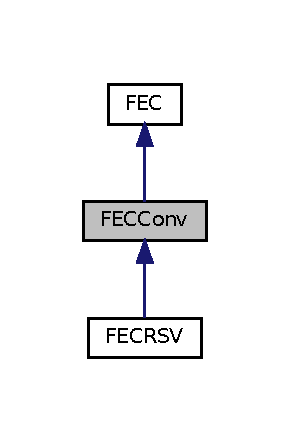
\includegraphics[width=140pt]{classFECConv__inherit__graph}
\end{center}
\end{figure}


Collaboration diagram for F\+E\+C\+Conv\+:
\nopagebreak
\begin{figure}[H]
\begin{center}
\leavevmode
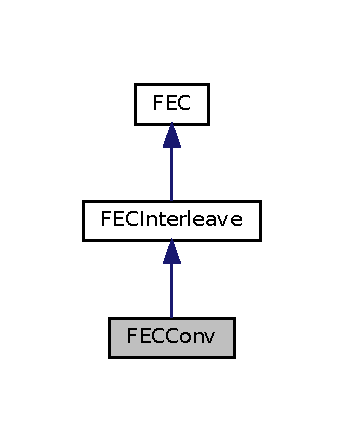
\includegraphics[width=140pt]{classFECConv__coll__graph}
\end{center}
\end{figure}
\doxysubsection*{Public Member Functions}
\begin{DoxyCompactItemize}
\item 
\mbox{\hyperlink{classFECConv_ac0159362b45b9f7840e3bf7223cd6e48}{F\+E\+C\+Conv}} (void)
\item 
\mbox{\hyperlink{classFECConv_a884d27178ca0484f4692b78fa31fd898}{F\+E\+C\+Conv}} (const size\+\_\+t inv\+\_\+rate, const size\+\_\+t order)
\item 
\mbox{\Hypertarget{classFECConv_a021d8db3fb79146d02b99015e4678ba4}\label{classFECConv_a021d8db3fb79146d02b99015e4678ba4}} 
\mbox{\hyperlink{classFECConv_a021d8db3fb79146d02b99015e4678ba4}{$\sim$\+F\+E\+C\+Conv}} (void)
\begin{DoxyCompactList}\small\item\em Destructor. \end{DoxyCompactList}\item 
size\+\_\+t \mbox{\hyperlink{classFECConv_a3b49acf69440d2677e3181513b9f3592}{get\+Enc\+Size}} (const size\+\_\+t msg\+\_\+len)
\item 
size\+\_\+t \mbox{\hyperlink{classFECConv_ae3e796d0e026dca718ed6384653a4564}{encode}} (const vector$<$ uint8\+\_\+t $>$ \&msg, vector$<$ uint8\+\_\+t $>$ \&enc\+\_\+msg)
\item 
ssize\+\_\+t \mbox{\hyperlink{classFECConv_afd897d6756bbbe4874942654e91a95e3}{decode}} (const vector$<$ uint8\+\_\+t $>$ \&enc\+\_\+msg, vector$<$ uint8\+\_\+t $>$ \&dec\+\_\+msg)
\end{DoxyCompactItemize}
\doxysubsection*{Protected Attributes}
\begin{DoxyCompactItemize}
\item 
\mbox{\Hypertarget{classFECConv_adbb15dc1ad17f9613559aa2527892be1}\label{classFECConv_adbb15dc1ad17f9613559aa2527892be1}} 
size\+\_\+t {\bfseries inv\+\_\+rate}
\item 
\mbox{\Hypertarget{classFECConv_aeb8954d7d5bd977494cca5a6a35a9dbc}\label{classFECConv_aeb8954d7d5bd977494cca5a6a35a9dbc}} 
size\+\_\+t {\bfseries order}
\item 
\mbox{\Hypertarget{classFECConv_a0978a376b15f30e89b8db481e229e0c7}\label{classFECConv_a0978a376b15f30e89b8db481e229e0c7}} 
correct\+\_\+convolutional $\ast$ {\bfseries corr\+\_\+con}
\end{DoxyCompactItemize}
\doxysubsection*{Additional Inherited Members}


\doxysubsection{Detailed Description}
Derived class that uses convolutional coding. 

\doxysubsection{Constructor \& Destructor Documentation}
\mbox{\Hypertarget{classFECConv_ac0159362b45b9f7840e3bf7223cd6e48}\label{classFECConv_ac0159362b45b9f7840e3bf7223cd6e48}} 
\index{FECConv@{FECConv}!FECConv@{FECConv}}
\index{FECConv@{FECConv}!FECConv@{FECConv}}
\doxysubsubsection{\texorpdfstring{FECConv()}{FECConv()}\hspace{0.1cm}{\footnotesize\ttfamily [1/2]}}
{\footnotesize\ttfamily F\+E\+C\+Conv\+::\+F\+E\+C\+Conv (\begin{DoxyParamCaption}\item[{void}]{ }\end{DoxyParamCaption})\hspace{0.3cm}{\ttfamily [inline]}}

Default constructor. Creates an \mbox{\hyperlink{classFECConv}{F\+E\+C\+Conv}} object with 1/2 rate and n=9. \mbox{\Hypertarget{classFECConv_a884d27178ca0484f4692b78fa31fd898}\label{classFECConv_a884d27178ca0484f4692b78fa31fd898}} 
\index{FECConv@{FECConv}!FECConv@{FECConv}}
\index{FECConv@{FECConv}!FECConv@{FECConv}}
\doxysubsubsection{\texorpdfstring{FECConv()}{FECConv()}\hspace{0.1cm}{\footnotesize\ttfamily [2/2]}}
{\footnotesize\ttfamily F\+E\+C\+Conv\+::\+F\+E\+C\+Conv (\begin{DoxyParamCaption}\item[{const size\+\_\+t}]{inv\+\_\+rate,  }\item[{const size\+\_\+t}]{order }\end{DoxyParamCaption})}

Constructor parameterizable with coding rate and order. 
\begin{DoxyParams}{Parameters}
{\em inv\+\_\+rate} & Coding rate. 2 and 3 are currently the only rates implemented. \\
\hline
{\em order} & Order of the coder. Values supported are 6, 7, 8, and 9. \\
\hline
\end{DoxyParams}


\doxysubsection{Member Function Documentation}
\mbox{\Hypertarget{classFECConv_afd897d6756bbbe4874942654e91a95e3}\label{classFECConv_afd897d6756bbbe4874942654e91a95e3}} 
\index{FECConv@{FECConv}!decode@{decode}}
\index{decode@{decode}!FECConv@{FECConv}}
\doxysubsubsection{\texorpdfstring{decode()}{decode()}}
{\footnotesize\ttfamily ssize\+\_\+t F\+E\+C\+Conv\+::decode (\begin{DoxyParamCaption}\item[{const vector$<$ uint8\+\_\+t $>$ \&}]{enc\+\_\+msg,  }\item[{vector$<$ uint8\+\_\+t $>$ \&}]{dec\+\_\+msg }\end{DoxyParamCaption})\hspace{0.3cm}{\ttfamily [virtual]}}

Decode F\+E\+C-\/coded data. Returns the decoded data size, in bytes. 
\begin{DoxyParams}{Parameters}
{\em enc\+\_\+msg} & Byte vector of encoded data. \\
\hline
{\em dec\+\_\+msg} & Byte vector of decoded data. \\
\hline
\end{DoxyParams}


Reimplemented from \mbox{\hyperlink{classFEC_aec87f2d9c2305283d226197bf76891cf}{F\+EC}}.



Reimplemented in \mbox{\hyperlink{classFECRSV_a4781900bd59579d7a380687c59179ae5}{F\+E\+C\+R\+SV}}.

\mbox{\Hypertarget{classFECConv_ae3e796d0e026dca718ed6384653a4564}\label{classFECConv_ae3e796d0e026dca718ed6384653a4564}} 
\index{FECConv@{FECConv}!encode@{encode}}
\index{encode@{encode}!FECConv@{FECConv}}
\doxysubsubsection{\texorpdfstring{encode()}{encode()}}
{\footnotesize\ttfamily size\+\_\+t F\+E\+C\+Conv\+::encode (\begin{DoxyParamCaption}\item[{const vector$<$ uint8\+\_\+t $>$ \&}]{msg,  }\item[{vector$<$ uint8\+\_\+t $>$ \&}]{enc\+\_\+msg }\end{DoxyParamCaption})\hspace{0.3cm}{\ttfamily [virtual]}}

Apply the \mbox{\hyperlink{classFEC}{F\+EC}} coding. Returns the encoded size, in bytes. 
\begin{DoxyParams}{Parameters}
{\em msg} & Byte vector of data to be encoded. \\
\hline
{\em enc\+\_\+msg} & Byte vector of encoded data. \\
\hline
\end{DoxyParams}


Reimplemented from \mbox{\hyperlink{classFEC_abc86f45390c50b3cd90cade73a137355}{F\+EC}}.



Reimplemented in \mbox{\hyperlink{classFECRSV_ac9bd3fe4c494067e6f24a1287b0c562e}{F\+E\+C\+R\+SV}}.

\mbox{\Hypertarget{classFECConv_a3b49acf69440d2677e3181513b9f3592}\label{classFECConv_a3b49acf69440d2677e3181513b9f3592}} 
\index{FECConv@{FECConv}!getEncSize@{getEncSize}}
\index{getEncSize@{getEncSize}!FECConv@{FECConv}}
\doxysubsubsection{\texorpdfstring{getEncSize()}{getEncSize()}}
{\footnotesize\ttfamily size\+\_\+t F\+E\+C\+Conv\+::get\+Enc\+Size (\begin{DoxyParamCaption}\item[{const size\+\_\+t}]{msg\+\_\+len }\end{DoxyParamCaption})\hspace{0.3cm}{\ttfamily [virtual]}}

Get the encoded size. 
\begin{DoxyParams}{Parameters}
{\em msg\+\_\+len} & The unencoded size of the message. \\
\hline
\end{DoxyParams}


Reimplemented from \mbox{\hyperlink{classFEC_a6504a5f7d5e1344538c25ed5481d0adb}{F\+EC}}.



Reimplemented in \mbox{\hyperlink{classFECRSV_a62fb01c152dad2e043ae75bbacfd928c}{F\+E\+C\+R\+SV}}.



The documentation for this class was generated from the following files\+:\begin{DoxyCompactItemize}
\item 
inc/protocol/fec.\+hpp\item 
src/protocol/fec.\+cpp\end{DoxyCompactItemize}

\hypertarget{classFECInterleave}{}\section{F\+E\+C\+Interleave Class Reference}
\label{classFECInterleave}\index{F\+E\+C\+Interleave@{F\+E\+C\+Interleave}}


Inheritance diagram for F\+E\+C\+Interleave\+:
\nopagebreak
\begin{figure}[H]
\begin{center}
\leavevmode
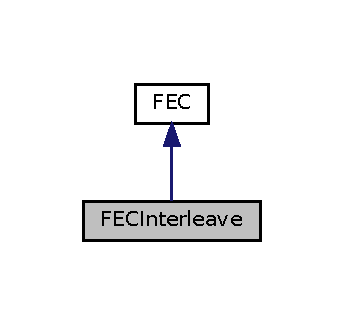
\includegraphics[width=164pt]{classFECInterleave__inherit__graph}
\end{center}
\end{figure}


Collaboration diagram for F\+E\+C\+Interleave\+:
\nopagebreak
\begin{figure}[H]
\begin{center}
\leavevmode
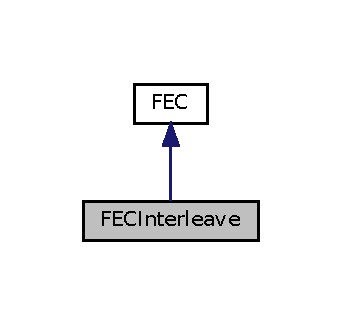
\includegraphics[width=164pt]{classFECInterleave__coll__graph}
\end{center}
\end{figure}
\subsection*{Public Member Functions}
\begin{DoxyCompactItemize}
\item 
\mbox{\Hypertarget{classFECInterleave_a10d868d7b117193667d0406edec2ef59}\label{classFECInterleave_a10d868d7b117193667d0406edec2ef59}} 
size\+\_\+t {\bfseries encode} (const vector$<$ uint8\+\_\+t $>$ \&msg, vector$<$ uint8\+\_\+t $>$ \&enc\+\_\+msg)
\item 
\mbox{\Hypertarget{classFECInterleave_a7e45a890ff7061e0a5c3234d29ac8954}\label{classFECInterleave_a7e45a890ff7061e0a5c3234d29ac8954}} 
ssize\+\_\+t {\bfseries decode} (const vector$<$ uint8\+\_\+t $>$ \&enc\+\_\+msg, vector$<$ uint8\+\_\+t $>$ \&dec\+\_\+msg)
\end{DoxyCompactItemize}
\subsection*{Additional Inherited Members}


The documentation for this class was generated from the following file\+:\begin{DoxyCompactItemize}
\item 
inc/protocol/fec.\+hpp\end{DoxyCompactItemize}

\hypertarget{classFECPolar}{}\section{F\+E\+C\+Polar Class Reference}
\label{classFECPolar}\index{F\+E\+C\+Polar@{F\+E\+C\+Polar}}


Inheritance diagram for F\+E\+C\+Polar\+:
\nopagebreak
\begin{figure}[H]
\begin{center}
\leavevmode
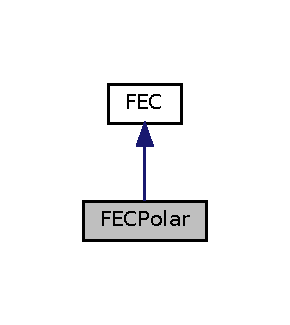
\includegraphics[width=139pt]{classFECPolar__inherit__graph}
\end{center}
\end{figure}


Collaboration diagram for F\+E\+C\+Polar\+:
\nopagebreak
\begin{figure}[H]
\begin{center}
\leavevmode
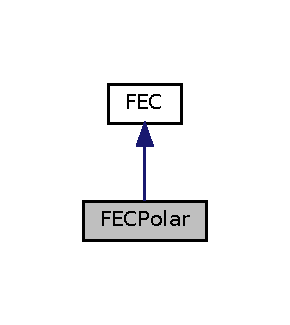
\includegraphics[width=139pt]{classFECPolar__coll__graph}
\end{center}
\end{figure}
\subsection*{Public Member Functions}
\begin{DoxyCompactItemize}
\item 
\mbox{\Hypertarget{classFECPolar_a7c62c4474b6a7ecd9dc897329e864096}\label{classFECPolar_a7c62c4474b6a7ecd9dc897329e864096}} 
{\bfseries F\+E\+C\+Polar} (const size\+\_\+t my\+\_\+block\+\_\+length, const size\+\_\+t my\+\_\+info\+\_\+length, const size\+\_\+t my\+\_\+list\+\_\+size)
\item 
\mbox{\Hypertarget{classFECPolar_a8589865e91e8ef0eed7bb440a445eb99}\label{classFECPolar_a8589865e91e8ef0eed7bb440a445eb99}} 
size\+\_\+t {\bfseries get\+Enc\+Size} (const size\+\_\+t msg\+\_\+len)
\item 
\mbox{\Hypertarget{classFECPolar_ab5662e1c2d45aa924936969261eb6faf}\label{classFECPolar_ab5662e1c2d45aa924936969261eb6faf}} 
size\+\_\+t {\bfseries encode} (const vector$<$ uint8\+\_\+t $>$ \&msg, vector$<$ uint8\+\_\+t $>$ \&enc\+\_\+msg)
\item 
\mbox{\Hypertarget{classFECPolar_adcf71d5e725bffa9b6e4c776eb8d4760}\label{classFECPolar_adcf71d5e725bffa9b6e4c776eb8d4760}} 
ssize\+\_\+t {\bfseries decode} (const vector$<$ uint8\+\_\+t $>$ \&enc\+\_\+msg, vector$<$ uint8\+\_\+t $>$ \&dec\+\_\+msg)
\item 
\mbox{\Hypertarget{classFECPolar_a897d3f06d446bf82f553d966a4725e6c}\label{classFECPolar_a897d3f06d446bf82f553d966a4725e6c}} 
ssize\+\_\+t {\bfseries decode\+Soft} (const vector$<$ uint8\+\_\+t $>$ \&enc\+\_\+msg, vector$<$ uint8\+\_\+t $>$ \&dec\+\_\+msg, const float snr)
\end{DoxyCompactItemize}
\subsection*{Protected Attributes}
\begin{DoxyCompactItemize}
\item 
\mbox{\Hypertarget{classFECPolar_aa919bab40c4d8d1c2fe86dea70b6e73b}\label{classFECPolar_aa919bab40c4d8d1c2fe86dea70b6e73b}} 
shared\+\_\+ptr$<$ Polar\+Code\+Lib\+::\+Polar\+Code $>$ {\bfseries polar\+\_\+code}
\item 
\mbox{\Hypertarget{classFECPolar_ab7147d119e70f8544871358e5520ac3f}\label{classFECPolar_ab7147d119e70f8544871358e5520ac3f}} 
size\+\_\+t {\bfseries block\+\_\+length}
\item 
\mbox{\Hypertarget{classFECPolar_ae2639cda67ff123d5b523ac6a2c242a0}\label{classFECPolar_ae2639cda67ff123d5b523ac6a2c242a0}} 
size\+\_\+t {\bfseries info\+\_\+length}
\item 
\mbox{\Hypertarget{classFECPolar_a84f2200d4fa1b44d67ae5c06d03116bc}\label{classFECPolar_a84f2200d4fa1b44d67ae5c06d03116bc}} 
size\+\_\+t {\bfseries list\+\_\+size}
\end{DoxyCompactItemize}
\subsection*{Additional Inherited Members}


The documentation for this class was generated from the following file\+:\begin{DoxyCompactItemize}
\item 
inc/protocol/fec.\+hpp\end{DoxyCompactItemize}

\hypertarget{classFECRSV}{}\doxysection{F\+E\+C\+R\+SV Class Reference}
\label{classFECRSV}\index{FECRSV@{FECRSV}}


{\ttfamily \#include $<$fec.\+hpp$>$}



Inheritance diagram for F\+E\+C\+R\+SV\+:\nopagebreak
\begin{figure}[H]
\begin{center}
\leavevmode
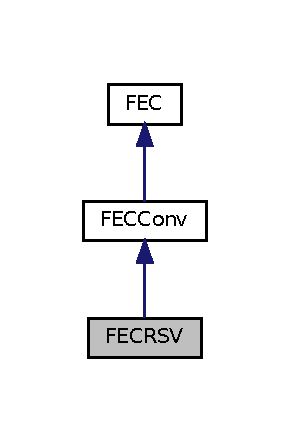
\includegraphics[width=165pt]{classFECRSV__inherit__graph}
\end{center}
\end{figure}


Collaboration diagram for F\+E\+C\+R\+SV\+:\nopagebreak
\begin{figure}[H]
\begin{center}
\leavevmode
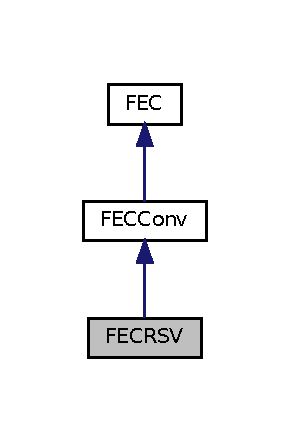
\includegraphics[width=165pt]{classFECRSV__coll__graph}
\end{center}
\end{figure}
\doxysubsection*{Public Member Functions}
\begin{DoxyCompactItemize}
\item 
\mbox{\hyperlink{classFECRSV_aa03ae357351b8428a28c3b72f9225c81}{F\+E\+C\+R\+SV}} (const int32\+\_\+t my\+\_\+msg\+\_\+len, const int32\+\_\+t inv\+\_\+rate, const int32\+\_\+t order, const int32\+\_\+t my\+\_\+rs\+\_\+corr\+\_\+bytes)
\item 
\mbox{\hyperlink{classFECRSV_aa43088e55ff0f57eb0b54e6d31ee679f}{F\+E\+C\+R\+SV}} (const int32\+\_\+t my\+\_\+msg\+\_\+len)
\item 
\mbox{\Hypertarget{classFECRSV_a5bfac8acff2c5604b4aa78417cceec5b}\label{classFECRSV_a5bfac8acff2c5604b4aa78417cceec5b}} 
\mbox{\hyperlink{classFECRSV_a5bfac8acff2c5604b4aa78417cceec5b}{$\sim$\+F\+E\+C\+R\+SV}} (void)
\begin{DoxyCompactList}\small\item\em Destructor. \end{DoxyCompactList}\item 
int32\+\_\+t \mbox{\hyperlink{classFECRSV_ae380d2a02345562d7174ab7f8dc8d192}{encode}} (const vector$<$ uint8\+\_\+t $>$ \&msg, vector$<$ uint8\+\_\+t $>$ \&rsv\+\_\+enc\+\_\+msg)
\item 
int32\+\_\+t \mbox{\hyperlink{classFECRSV_a2eb1f75ca4d24879c3ec89b5358d8291}{decode}} (const vector$<$ uint8\+\_\+t $>$ \&rsv\+\_\+enc\+\_\+msg, vector$<$ uint8\+\_\+t $>$ \&dec\+\_\+msg)
\end{DoxyCompactItemize}
\doxysubsection*{Protected Attributes}
\begin{DoxyCompactItemize}
\item 
\mbox{\Hypertarget{classFECRSV_a075caf63c36bda24893e913cd301b7f3}\label{classFECRSV_a075caf63c36bda24893e913cd301b7f3}} 
int32\+\_\+t {\bfseries rs\+\_\+corr\+\_\+bytes}
\item 
\mbox{\Hypertarget{classFECRSV_a6032e72eb4d7e2256009769bba63b9b7}\label{classFECRSV_a6032e72eb4d7e2256009769bba63b9b7}} 
correct\+\_\+reed\+\_\+solomon $\ast$ {\bfseries rs\+\_\+con}
\item 
\mbox{\Hypertarget{classFECRSV_af90e5fbf723f969ce99406391b8619c4}\label{classFECRSV_af90e5fbf723f969ce99406391b8619c4}} 
int32\+\_\+t {\bfseries rs\+\_\+enc\+\_\+msg\+\_\+size}
\end{DoxyCompactItemize}
\doxysubsection*{Additional Inherited Members}


\doxysubsection{Detailed Description}
Derived class that implements Reed-\/\+Solomon-\/\+Viterbi (R\+SV) forward error correction. The convolutional coding is the same as implemented in the \mbox{\hyperlink{classFECConv}{F\+E\+C\+Conv}} class, and the Reed-\/\+Solomon outer code is a (256,223) code. 

\doxysubsection{Constructor \& Destructor Documentation}
\mbox{\Hypertarget{classFECRSV_aa03ae357351b8428a28c3b72f9225c81}\label{classFECRSV_aa03ae357351b8428a28c3b72f9225c81}} 
\index{FECRSV@{FECRSV}!FECRSV@{FECRSV}}
\index{FECRSV@{FECRSV}!FECRSV@{FECRSV}}
\doxysubsubsection{\texorpdfstring{FECRSV()}{FECRSV()}\hspace{0.1cm}{\footnotesize\ttfamily [1/2]}}
{\footnotesize\ttfamily F\+E\+C\+R\+S\+V\+::\+F\+E\+C\+R\+SV (\begin{DoxyParamCaption}\item[{const int32\+\_\+t}]{my\+\_\+msg\+\_\+len,  }\item[{const int32\+\_\+t}]{inv\+\_\+rate,  }\item[{const int32\+\_\+t}]{order,  }\item[{const int32\+\_\+t}]{my\+\_\+rs\+\_\+corr\+\_\+bytes }\end{DoxyParamCaption})}

Constructor. 
\begin{DoxyParams}{Parameters}
{\em inv\+\_\+rate} & Convolutional coding rate. \\
\hline
{\em order} & Convolutional coding order. \\
\hline
{\em my\+\_\+rs\+\_\+corr\+\_\+bytes} & Number of Reed-\/\+Solomon correction bytes. \\
\hline
\end{DoxyParams}
\mbox{\Hypertarget{classFECRSV_aa43088e55ff0f57eb0b54e6d31ee679f}\label{classFECRSV_aa43088e55ff0f57eb0b54e6d31ee679f}} 
\index{FECRSV@{FECRSV}!FECRSV@{FECRSV}}
\index{FECRSV@{FECRSV}!FECRSV@{FECRSV}}
\doxysubsubsection{\texorpdfstring{FECRSV()}{FECRSV()}\hspace{0.1cm}{\footnotesize\ttfamily [2/2]}}
{\footnotesize\ttfamily F\+E\+C\+R\+S\+V\+::\+F\+E\+C\+R\+SV (\begin{DoxyParamCaption}\item[{const int32\+\_\+t}]{my\+\_\+msg\+\_\+len }\end{DoxyParamCaption})\hspace{0.3cm}{\ttfamily [inline]}}

Default constructor. Initializes with a convolutional coding rate of 2, n=9, and 32 Reed-\/\+Solomon correction bytes. 

\doxysubsection{Member Function Documentation}
\mbox{\Hypertarget{classFECRSV_a2eb1f75ca4d24879c3ec89b5358d8291}\label{classFECRSV_a2eb1f75ca4d24879c3ec89b5358d8291}} 
\index{FECRSV@{FECRSV}!decode@{decode}}
\index{decode@{decode}!FECRSV@{FECRSV}}
\doxysubsubsection{\texorpdfstring{decode()}{decode()}}
{\footnotesize\ttfamily int32\+\_\+t F\+E\+C\+R\+S\+V\+::decode (\begin{DoxyParamCaption}\item[{const vector$<$ uint8\+\_\+t $>$ \&}]{enc\+\_\+msg,  }\item[{vector$<$ uint8\+\_\+t $>$ \&}]{dec\+\_\+msg }\end{DoxyParamCaption})\hspace{0.3cm}{\ttfamily [virtual]}}

Decode F\+E\+C-\/coded data. Returns the decoded data size, in bytes. 
\begin{DoxyParams}{Parameters}
{\em enc\+\_\+msg} & Byte vector of encoded data. \\
\hline
{\em dec\+\_\+msg} & Byte vector of decoded data. \\
\hline
\end{DoxyParams}


Reimplemented from \mbox{\hyperlink{classFECConv_a6bec28009aa10bbf34f13b3f3f9315fe}{F\+E\+C\+Conv}}.

\mbox{\Hypertarget{classFECRSV_ae380d2a02345562d7174ab7f8dc8d192}\label{classFECRSV_ae380d2a02345562d7174ab7f8dc8d192}} 
\index{FECRSV@{FECRSV}!encode@{encode}}
\index{encode@{encode}!FECRSV@{FECRSV}}
\doxysubsubsection{\texorpdfstring{encode()}{encode()}}
{\footnotesize\ttfamily int32\+\_\+t F\+E\+C\+R\+S\+V\+::encode (\begin{DoxyParamCaption}\item[{const vector$<$ uint8\+\_\+t $>$ \&}]{msg,  }\item[{vector$<$ uint8\+\_\+t $>$ \&}]{enc\+\_\+msg }\end{DoxyParamCaption})\hspace{0.3cm}{\ttfamily [virtual]}}

Apply the \mbox{\hyperlink{classFEC}{F\+EC}} coding. Returns the encoded size, in bytes. 
\begin{DoxyParams}{Parameters}
{\em msg} & Byte vector of data to be encoded. \\
\hline
{\em enc\+\_\+msg} & Byte vector of encoded data. \\
\hline
\end{DoxyParams}


Reimplemented from \mbox{\hyperlink{classFECConv_a00c8d7fb39380c66a5038d288179587d}{F\+E\+C\+Conv}}.



The documentation for this class was generated from the following files\+:\begin{DoxyCompactItemize}
\item 
inc/protocol/fec.\+hpp\item 
src/protocol/fec.\+cpp\end{DoxyCompactItemize}

\hypertarget{classFrame}{}\doxysection{Frame Class Reference}
\label{classFrame}\index{Frame@{Frame}}


{\ttfamily \#include $<$serial\+\_\+data.\+hpp$>$}



Collaboration diagram for Frame\+:\nopagebreak
\begin{figure}[H]
\begin{center}
\leavevmode
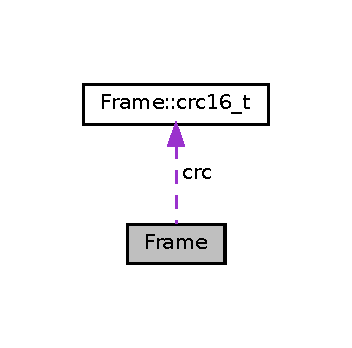
\includegraphics[width=169pt]{classFrame__coll__graph}
\end{center}
\end{figure}
\doxysubsection*{Classes}
\begin{DoxyCompactItemize}
\item 
union \mbox{\hyperlink{unionFrame_1_1crc16__t}{crc16\+\_\+t}}
\end{DoxyCompactItemize}
\doxysubsection*{Public Member Functions}
\begin{DoxyCompactItemize}
\item 
\mbox{\Hypertarget{classFrame_a1c9286c3bbd1c0393baefa0ee4120a04}\label{classFrame_a1c9286c3bbd1c0393baefa0ee4120a04}} 
struct {\bfseries \+\_\+\+\_\+attribute\+\_\+\+\_\+} ((\+\_\+\+\_\+packed\+\_\+\+\_\+))
\item 
\mbox{\hyperlink{classFrame_ad2e5946cf41d4817e750500acf05d02b}{Frame}} ()
\item 
\mbox{\hyperlink{classFrame_a230b093686859a8d614b81b19f0433a0}{Frame}} (shared\+\_\+ptr$<$ \mbox{\hyperlink{classFEC}{F\+EC}} $>$ my\+\_\+fec)
\item 
\mbox{\Hypertarget{classFrame_abc897b6f22eabc8d4b2f12821bce1649}\label{classFrame_abc897b6f22eabc8d4b2f12821bce1649}} 
void {\bfseries serialize} (vector$<$ uint8\+\_\+t $>$ \&ser\+\_\+frame)
\item 
\mbox{\Hypertarget{classFrame_a40746b6fa955619e185573c1d38022dd}\label{classFrame_a40746b6fa955619e185573c1d38022dd}} 
bool \mbox{\hyperlink{classFrame_a40746b6fa955619e185573c1d38022dd}{operator==}} (const \mbox{\hyperlink{classFrame}{Frame}} \&L)
\begin{DoxyCompactList}\small\item\em Equality operator for Frames. \end{DoxyCompactList}\item 
\mbox{\Hypertarget{classFrame_a604c4dc3f60c7bf4e861243f05ace9b8}\label{classFrame_a604c4dc3f60c7bf4e861243f05ace9b8}} 
bool \mbox{\hyperlink{classFrame_a604c4dc3f60c7bf4e861243f05ace9b8}{operator!=}} (const \mbox{\hyperlink{classFrame}{Frame}} \&L)
\begin{DoxyCompactList}\small\item\em Inequality operator for Frames. \end{DoxyCompactList}\item 
void \mbox{\hyperlink{classFrame_ae0082da89627bc112701735227104eec}{load\+Test\+Frame}} (vector$<$ uint8\+\_\+t $>$ \&buf)
\item 
size\+\_\+t \mbox{\hyperlink{classFrame_a57812c04330da0044155af6e2ca9a6a7}{get\+Payload}} (vector$<$ uint8\+\_\+t $>$ \&buf)
\item 
size\+\_\+t \mbox{\hyperlink{classFrame_a950b26a59c2f2716662a09964e5d95d1}{set\+Beacon\+Payload}} (string \&beacon\+\_\+str)
\item 
\mbox{\Hypertarget{classFrame_ad72ae3be73f6ef1ac0db92014f7eda7f}\label{classFrame_ad72ae3be73f6ef1ac0db92014f7eda7f}} 
void {\bfseries whiten} (const vector$<$ uint8\+\_\+t $>$ \&buf, vector$<$ uint8\+\_\+t $>$ \&wht\+\_\+buf, const uint16\+\_\+t seed)
\item 
size\+\_\+t \mbox{\hyperlink{classFrame_a2e1d5421694ec4d9abaadacf2b32b492}{serialize\+Coded}} (vector$<$ uint8\+\_\+t $>$ \&buf)
\item 
uint16\+\_\+t \mbox{\hyperlink{classFrame_a84bdc2969f8962206c89c5f916d80973}{calc\+C\+RC}} (void)
\item 
uint32\+\_\+t \mbox{\hyperlink{classFrame_a690b8728c8215af874f0aed2c643d7a6}{calc\+Unique\+C\+RC}} (void)
\item 
bool \mbox{\hyperlink{classFrame_a99bf5c1a41572292c07bc9699a491a96}{check\+C\+RC}} (void)
\item 
uint16\+\_\+t \mbox{\hyperlink{classFrame_aa2de2dba681188cc6ab00dfc42d15426}{set\+C\+RC}} (void)
\item 
void \mbox{\hyperlink{classFrame_a982cef0e09413cc2a5c55298e2cc7c5f}{set\+Sender}} (uint8\+\_\+t sender\+\_\+addr)
\item 
uint32\+\_\+t \mbox{\hyperlink{classFrame_a278632174fa07b44e0dabda3d010f000}{get\+Sender}} (void)
\item 
void \mbox{\hyperlink{classFrame_af3cc33a2ea60ad84db23097da6df3c31}{set\+Stream\+ID}} (uint8\+\_\+t id)
\item 
uint32\+\_\+t \mbox{\hyperlink{classFrame_ad98ec7af45ce4428441d2ee3d28bae7e}{get\+Stream\+ID}} (void)
\item 
P\+K\+T\+\_\+\+S\+T\+A\+T\+U\+S\+\_\+\+E\+N\+UM \mbox{\hyperlink{classFrame_a448b698fd4cc568e610f87f971354dc6}{deserialize\+Coded}} (const shared\+\_\+ptr$<$ vector$<$ uint8\+\_\+t $>$$>$ buf)
\item 
void \mbox{\hyperlink{classFrame_a46139e40aaadc65459f1d094e6f7fc20}{increment\+T\+TL}} (void)
\item 
uint8\+\_\+t \mbox{\hyperlink{classFrame_a383e2fb65096f4c57f37b48d3d74f07d}{get\+T\+TL}} (void)
\item 
size\+\_\+t \mbox{\hyperlink{classFrame_a14c155e1ec94aa20bec722efaff3b25d}{coded\+Size}} (void)
\item 
void \mbox{\hyperlink{classFrame_ac93b8d79eb8cf07459bab3ef49ddb6e8}{get\+Offsets}} (uint8\+\_\+t \&pre\+\_\+offset, uint8\+\_\+t \&nsym\+\_\+offset, uint8\+\_\+t \&sym\+\_\+offset)
\item 
void \mbox{\hyperlink{classFrame_ad49bfde5dc426762cc1058b95052ca70}{set\+Offsets}} (const uint8\+\_\+t pre\+\_\+offset, const uint8\+\_\+t nsym\+\_\+offset, const uint8\+\_\+t sym\+\_\+offset)
\item 
void \mbox{\hyperlink{classFrame_a1caeb909554201233a464f24e445a5e1}{get\+Rx\+Stats}} (int16\+\_\+t \&rssi, int8\+\_\+t \&snr, uint16\+\_\+t \&rx\+\_\+size)
\item 
void \mbox{\hyperlink{classFrame_a6f48959a7d7971ad25d25bf5c5237b22}{set\+Rx\+Stats}} (const int16\+\_\+t rssi, const int8\+\_\+t snr, const uint16\+\_\+t rx\+\_\+size)
\item 
uint16\+\_\+t \mbox{\hyperlink{classFrame_ab6513ed996012cf14141615c1ed47e38}{get\+C\+RC}} (void)
\item 
void \mbox{\hyperlink{classFrame_a6fba80bf6639a27ffffb612e64cf6844}{pretty\+Print}} (const enum D\+B\+G\+\_\+\+T\+Y\+P\+ES dbg\+\_\+type)
\item 
void \mbox{\hyperlink{classFrame_a2ef721542c17f972913df4375d72f7bf}{load\+From\+J\+S\+ON}} (Mbed\+J\+S\+O\+N\+Value \&json)
\item 
void \mbox{\hyperlink{classFrame_a865ca9d9a5584fab74d7258012509b97}{save\+To\+J\+S\+ON}} (Mbed\+J\+S\+O\+N\+Value \&json)
\end{DoxyCompactItemize}
\doxysubsection*{Static Public Member Functions}
\begin{DoxyCompactItemize}
\item 
static size\+\_\+t \mbox{\hyperlink{classFrame_aa38b49286989b869cd82ac064ead3628}{size}} (void)
\item 
static size\+\_\+t \mbox{\hyperlink{classFrame_a1807a7893ff81064f2e92cb5ab065ec8}{hdr\+Size}} (void)
\end{DoxyCompactItemize}
\doxysubsection*{Public Attributes}
\begin{DoxyCompactItemize}
\item 
\mbox{\Hypertarget{classFrame_aaaf5414ab06dbc255a62733d927807f4}\label{classFrame_aaaf5414ab06dbc255a62733d927807f4}} 
{\bfseries frame\+\_\+hdr}
\item 
\mbox{\Hypertarget{classFrame_a0a718492a654222c71e8ff0b8e06fb8a}\label{classFrame_a0a718492a654222c71e8ff0b8e06fb8a}} 
shared\+\_\+ptr$<$ \mbox{\hyperlink{classFEC}{F\+EC}} $>$ {\bfseries fec}
\item 
\mbox{\Hypertarget{classFrame_afc760f301f1c03205d4862bbaad0442a}\label{classFrame_afc760f301f1c03205d4862bbaad0442a}} 
bool {\bfseries tx\+\_\+frame}
\end{DoxyCompactItemize}
\doxysubsection*{Protected Attributes}
\begin{DoxyCompactItemize}
\item 
\mbox{\Hypertarget{classFrame_ab7a6e2ca6c4b411ff1f2152ec1261539}\label{classFrame_ab7a6e2ca6c4b411ff1f2152ec1261539}} 
int16\+\_\+t {\bfseries rssi}
\item 
\mbox{\Hypertarget{classFrame_a0bac5a6c745a0464b506884fe7ce4de4}\label{classFrame_a0bac5a6c745a0464b506884fe7ce4de4}} 
int8\+\_\+t {\bfseries snr}
\item 
\mbox{\Hypertarget{classFrame_a4f9076d957cbace63b33dea31746f266}\label{classFrame_a4f9076d957cbace63b33dea31746f266}} 
uint16\+\_\+t {\bfseries rx\+\_\+size}
\item 
\mbox{\Hypertarget{classFrame_adfe9288bf669e9ae08f61fa18b82c47f}\label{classFrame_adfe9288bf669e9ae08f61fa18b82c47f}} 
P\+K\+T\+\_\+\+S\+T\+A\+T\+U\+S\+\_\+\+E\+N\+UM {\bfseries pkt\+\_\+status}
\end{DoxyCompactItemize}
\doxysubsection*{Private Attributes}
\begin{DoxyCompactItemize}
\item 
\mbox{\Hypertarget{classFrame_ad08ba2f639e3c7d47cde39ecec16c4d3}\label{classFrame_ad08ba2f639e3c7d47cde39ecec16c4d3}} 
frame\+\_\+hdr {\bfseries hdr}
\item 
\mbox{\Hypertarget{classFrame_a0af26264fb9334282af8ad0ab6253bf0}\label{classFrame_a0af26264fb9334282af8ad0ab6253bf0}} 
vector$<$ uint8\+\_\+t $>$ {\bfseries data}
\item 
\mbox{\Hypertarget{classFrame_aeb9531efc4880ad98cce77dd266e2f74}\label{classFrame_aeb9531efc4880ad98cce77dd266e2f74}} 
\mbox{\hyperlink{unionFrame_1_1crc16__t}{crc16\+\_\+t}} {\bfseries crc}
\end{DoxyCompactItemize}


\doxysubsection{Detailed Description}
This class implements the Q\+Mesh \mbox{\hyperlink{classFrame}{Frame}}. It provides both the storage of \mbox{\hyperlink{classFrame}{Frame}} data fields as well as various methods for performing various functionality needed for Q\+Mesh, such as\+:
\begin{DoxyItemize}
\item Checksum (C\+RC) calculations
\item Time-\/to-\/\+Live (T\+TL) handling
\item \mbox{\hyperlink{classFEC}{F\+EC}} encoding/decoding
\item Serialization/deserialization 
\end{DoxyItemize}

\doxysubsection{Constructor \& Destructor Documentation}
\mbox{\Hypertarget{classFrame_ad2e5946cf41d4817e750500acf05d02b}\label{classFrame_ad2e5946cf41d4817e750500acf05d02b}} 
\index{Frame@{Frame}!Frame@{Frame}}
\index{Frame@{Frame}!Frame@{Frame}}
\doxysubsubsection{\texorpdfstring{Frame()}{Frame()}\hspace{0.1cm}{\footnotesize\ttfamily [1/2]}}
{\footnotesize\ttfamily Frame\+::\+Frame (\begin{DoxyParamCaption}{ }\end{DoxyParamCaption})\hspace{0.3cm}{\ttfamily [inline]}}

Default constructor. Constructs with a default \mbox{\hyperlink{classFEC}{F\+EC}} (one that does nothing). \mbox{\Hypertarget{classFrame_a230b093686859a8d614b81b19f0433a0}\label{classFrame_a230b093686859a8d614b81b19f0433a0}} 
\index{Frame@{Frame}!Frame@{Frame}}
\index{Frame@{Frame}!Frame@{Frame}}
\doxysubsubsection{\texorpdfstring{Frame()}{Frame()}\hspace{0.1cm}{\footnotesize\ttfamily [2/2]}}
{\footnotesize\ttfamily Frame\+::\+Frame (\begin{DoxyParamCaption}\item[{shared\+\_\+ptr$<$ \mbox{\hyperlink{classFEC}{F\+EC}} $>$}]{my\+\_\+fec }\end{DoxyParamCaption})\hspace{0.3cm}{\ttfamily [inline]}}

Constructor that loads a specific \mbox{\hyperlink{classFEC}{F\+EC}}. 
\begin{DoxyParams}{Parameters}
{\em my\+\_\+fec} & shared\+\_\+ptr to the \mbox{\hyperlink{classFEC}{F\+EC}} object. \\
\hline
\end{DoxyParams}


\doxysubsection{Member Function Documentation}
\mbox{\Hypertarget{classFrame_a84bdc2969f8962206c89c5f916d80973}\label{classFrame_a84bdc2969f8962206c89c5f916d80973}} 
\index{Frame@{Frame}!calcCRC@{calcCRC}}
\index{calcCRC@{calcCRC}!Frame@{Frame}}
\doxysubsubsection{\texorpdfstring{calcCRC()}{calcCRC()}}
{\footnotesize\ttfamily uint16\+\_\+t Frame\+::calc\+C\+RC (\begin{DoxyParamCaption}\item[{void}]{ }\end{DoxyParamCaption})}

Calculate the C\+RC of the payload. \mbox{\Hypertarget{classFrame_a690b8728c8215af874f0aed2c643d7a6}\label{classFrame_a690b8728c8215af874f0aed2c643d7a6}} 
\index{Frame@{Frame}!calcUniqueCRC@{calcUniqueCRC}}
\index{calcUniqueCRC@{calcUniqueCRC}!Frame@{Frame}}
\doxysubsubsection{\texorpdfstring{calcUniqueCRC()}{calcUniqueCRC()}}
{\footnotesize\ttfamily uint32\+\_\+t Frame\+::calc\+Unique\+C\+RC (\begin{DoxyParamCaption}\item[{void}]{ }\end{DoxyParamCaption})}

Calculate the C\+RC for the \char`\"{}unique\char`\"{} information. The unique information consists of the type, stream\+\_\+id, and payload. This method is primarily used to provide a unique \char`\"{}hash\char`\"{} for Frames in order to determine whether the Q\+Mesh node has seen them before. \mbox{\Hypertarget{classFrame_a99bf5c1a41572292c07bc9699a491a96}\label{classFrame_a99bf5c1a41572292c07bc9699a491a96}} 
\index{Frame@{Frame}!checkCRC@{checkCRC}}
\index{checkCRC@{checkCRC}!Frame@{Frame}}
\doxysubsubsection{\texorpdfstring{checkCRC()}{checkCRC()}}
{\footnotesize\ttfamily bool Frame\+::check\+C\+RC (\begin{DoxyParamCaption}\item[{void}]{ }\end{DoxyParamCaption})\hspace{0.3cm}{\ttfamily [inline]}}

Check the payload C\+RC, returning True if a match, False if not. \mbox{\Hypertarget{classFrame_a14c155e1ec94aa20bec722efaff3b25d}\label{classFrame_a14c155e1ec94aa20bec722efaff3b25d}} 
\index{Frame@{Frame}!codedSize@{codedSize}}
\index{codedSize@{codedSize}!Frame@{Frame}}
\doxysubsubsection{\texorpdfstring{codedSize()}{codedSize()}}
{\footnotesize\ttfamily size\+\_\+t Frame\+::coded\+Size (\begin{DoxyParamCaption}\item[{void}]{ }\end{DoxyParamCaption})}

Get the size, in bytes, of a \mbox{\hyperlink{classFrame}{Frame}} after \mbox{\hyperlink{classFEC}{F\+EC}} encoding. \mbox{\Hypertarget{classFrame_a448b698fd4cc568e610f87f971354dc6}\label{classFrame_a448b698fd4cc568e610f87f971354dc6}} 
\index{Frame@{Frame}!deserializeCoded@{deserializeCoded}}
\index{deserializeCoded@{deserializeCoded}!Frame@{Frame}}
\doxysubsubsection{\texorpdfstring{deserializeCoded()}{deserializeCoded()}}
{\footnotesize\ttfamily P\+K\+T\+\_\+\+S\+T\+A\+T\+U\+S\+\_\+\+E\+N\+UM Frame\+::deserialize\+Coded (\begin{DoxyParamCaption}\item[{const shared\+\_\+ptr$<$ vector$<$ uint8\+\_\+t $>$$>$}]{buf }\end{DoxyParamCaption})}

Takes a vector of bytes and loads it into the \mbox{\hyperlink{classFrame}{Frame}}\textquotesingle{}s internal data structures. This is designed to take bytes received off the air, so it performs \mbox{\hyperlink{classFEC}{F\+EC}} decoding, and will return a P\+K\+T\+\_\+\+S\+T\+A\+T\+U\+S\+\_\+\+E\+N\+UM with the results (testing stuff out)\+: ~\newline

\begin{DoxyItemize}
\item P\+K\+T\+\_\+\+F\+E\+C\+\_\+\+F\+A\+IL -- \mbox{\hyperlink{classFEC}{F\+EC}} decoding failed ~\newline

\item P\+K\+T\+\_\+\+B\+A\+D\+\_\+\+S\+I\+ZE -- Packet size is inconsistent with bytes decoded ~\newline

\item P\+K\+T\+\_\+\+B\+A\+D\+\_\+\+C\+RC -- Bad packet payload C\+RC ~\newline

\item P\+K\+T\+\_\+\+OK -- Packet decoded successfully ~\newline
 
\begin{DoxyParams}{Parameters}
{\em buf} & shared\+\_\+ptr to a vector of received, encoded bytes to decode \\
\hline
\end{DoxyParams}

\end{DoxyItemize}\mbox{\Hypertarget{classFrame_ab6513ed996012cf14141615c1ed47e38}\label{classFrame_ab6513ed996012cf14141615c1ed47e38}} 
\index{Frame@{Frame}!getCRC@{getCRC}}
\index{getCRC@{getCRC}!Frame@{Frame}}
\doxysubsubsection{\texorpdfstring{getCRC()}{getCRC()}}
{\footnotesize\ttfamily uint16\+\_\+t Frame\+::get\+C\+RC (\begin{DoxyParamCaption}\item[{void}]{ }\end{DoxyParamCaption})\hspace{0.3cm}{\ttfamily [inline]}}

Returns the payload C\+RC stored within the \mbox{\hyperlink{classFrame}{Frame}} object. \mbox{\Hypertarget{classFrame_ac93b8d79eb8cf07459bab3ef49ddb6e8}\label{classFrame_ac93b8d79eb8cf07459bab3ef49ddb6e8}} 
\index{Frame@{Frame}!getOffsets@{getOffsets}}
\index{getOffsets@{getOffsets}!Frame@{Frame}}
\doxysubsubsection{\texorpdfstring{getOffsets()}{getOffsets()}}
{\footnotesize\ttfamily void Frame\+::get\+Offsets (\begin{DoxyParamCaption}\item[{uint8\+\_\+t \&}]{pre\+\_\+offset,  }\item[{uint8\+\_\+t \&}]{nsym\+\_\+offset,  }\item[{uint8\+\_\+t \&}]{sym\+\_\+offset }\end{DoxyParamCaption})\hspace{0.3cm}{\ttfamily [inline]}}

Get the offsets from the packet header 
\begin{DoxyParams}{Parameters}
{\em pre\+\_\+offset} & Number of preamble-\/length offsets \\
\hline
{\em nsym\+\_\+offset} & Number of symbol-\/length offsets \\
\hline
{\em sym\+\_\+offset} & Intra-\/symbol offset. \\
\hline
\end{DoxyParams}
\mbox{\Hypertarget{classFrame_a57812c04330da0044155af6e2ca9a6a7}\label{classFrame_a57812c04330da0044155af6e2ca9a6a7}} 
\index{Frame@{Frame}!getPayload@{getPayload}}
\index{getPayload@{getPayload}!Frame@{Frame}}
\doxysubsubsection{\texorpdfstring{getPayload()}{getPayload()}}
{\footnotesize\ttfamily size\+\_\+t Frame\+::get\+Payload (\begin{DoxyParamCaption}\item[{vector$<$ uint8\+\_\+t $>$ \&}]{buf }\end{DoxyParamCaption})\hspace{0.3cm}{\ttfamily [inline]}}

Get the payload. Returns the number of bytes in the payload. 
\begin{DoxyParams}{Parameters}
{\em buf} & Where the payload bytes are put. \\
\hline
\end{DoxyParams}
\mbox{\Hypertarget{classFrame_a1caeb909554201233a464f24e445a5e1}\label{classFrame_a1caeb909554201233a464f24e445a5e1}} 
\index{Frame@{Frame}!getRxStats@{getRxStats}}
\index{getRxStats@{getRxStats}!Frame@{Frame}}
\doxysubsubsection{\texorpdfstring{getRxStats()}{getRxStats()}}
{\footnotesize\ttfamily void Frame\+::get\+Rx\+Stats (\begin{DoxyParamCaption}\item[{int16\+\_\+t \&}]{rssi,  }\item[{int8\+\_\+t \&}]{snr,  }\item[{uint16\+\_\+t \&}]{rx\+\_\+size }\end{DoxyParamCaption})\hspace{0.3cm}{\ttfamily [inline]}}

Get the receive statistics 
\begin{DoxyParams}{Parameters}
{\em rssi} & Full-\/packet R\+S\+SI \\
\hline
{\em snr} & Full-\/packet S\+NR \\
\hline
{\em rx\+\_\+size} & Number of bytes received \\
\hline
\end{DoxyParams}
\mbox{\Hypertarget{classFrame_a278632174fa07b44e0dabda3d010f000}\label{classFrame_a278632174fa07b44e0dabda3d010f000}} 
\index{Frame@{Frame}!getSender@{getSender}}
\index{getSender@{getSender}!Frame@{Frame}}
\doxysubsubsection{\texorpdfstring{getSender()}{getSender()}}
{\footnotesize\ttfamily uint32\+\_\+t Frame\+::get\+Sender (\begin{DoxyParamCaption}\item[{void}]{ }\end{DoxyParamCaption})\hspace{0.3cm}{\ttfamily [inline]}}

Gets the sender\textquotesingle{}s address. \mbox{\Hypertarget{classFrame_ad98ec7af45ce4428441d2ee3d28bae7e}\label{classFrame_ad98ec7af45ce4428441d2ee3d28bae7e}} 
\index{Frame@{Frame}!getStreamID@{getStreamID}}
\index{getStreamID@{getStreamID}!Frame@{Frame}}
\doxysubsubsection{\texorpdfstring{getStreamID()}{getStreamID()}}
{\footnotesize\ttfamily uint32\+\_\+t Frame\+::get\+Stream\+ID (\begin{DoxyParamCaption}\item[{void}]{ }\end{DoxyParamCaption})\hspace{0.3cm}{\ttfamily [inline]}}

Returns the Stream ID \mbox{\Hypertarget{classFrame_a383e2fb65096f4c57f37b48d3d74f07d}\label{classFrame_a383e2fb65096f4c57f37b48d3d74f07d}} 
\index{Frame@{Frame}!getTTL@{getTTL}}
\index{getTTL@{getTTL}!Frame@{Frame}}
\doxysubsubsection{\texorpdfstring{getTTL()}{getTTL()}}
{\footnotesize\ttfamily uint8\+\_\+t Frame\+::get\+T\+TL (\begin{DoxyParamCaption}\item[{void}]{ }\end{DoxyParamCaption})\hspace{0.3cm}{\ttfamily [inline]}}

Return the frame\textquotesingle{}s current T\+TL value \mbox{\Hypertarget{classFrame_a1807a7893ff81064f2e92cb5ab065ec8}\label{classFrame_a1807a7893ff81064f2e92cb5ab065ec8}} 
\index{Frame@{Frame}!hdrSize@{hdrSize}}
\index{hdrSize@{hdrSize}!Frame@{Frame}}
\doxysubsubsection{\texorpdfstring{hdrSize()}{hdrSize()}}
{\footnotesize\ttfamily static size\+\_\+t Frame\+::hdr\+Size (\begin{DoxyParamCaption}\item[{void}]{ }\end{DoxyParamCaption})\hspace{0.3cm}{\ttfamily [inline]}, {\ttfamily [static]}}

Returns the size of a packet header \mbox{\Hypertarget{classFrame_a46139e40aaadc65459f1d094e6f7fc20}\label{classFrame_a46139e40aaadc65459f1d094e6f7fc20}} 
\index{Frame@{Frame}!incrementTTL@{incrementTTL}}
\index{incrementTTL@{incrementTTL}!Frame@{Frame}}
\doxysubsubsection{\texorpdfstring{incrementTTL()}{incrementTTL()}}
{\footnotesize\ttfamily void Frame\+::increment\+T\+TL (\begin{DoxyParamCaption}\item[{void}]{ }\end{DoxyParamCaption})\hspace{0.3cm}{\ttfamily [inline]}}

Increment the T\+TL, updating the header C\+RC in the process. \mbox{\Hypertarget{classFrame_a2ef721542c17f972913df4375d72f7bf}\label{classFrame_a2ef721542c17f972913df4375d72f7bf}} 
\index{Frame@{Frame}!loadFromJSON@{loadFromJSON}}
\index{loadFromJSON@{loadFromJSON}!Frame@{Frame}}
\doxysubsubsection{\texorpdfstring{loadFromJSON()}{loadFromJSON()}}
{\footnotesize\ttfamily void Frame\+::load\+From\+J\+S\+ON (\begin{DoxyParamCaption}\item[{Mbed\+J\+S\+O\+N\+Value \&}]{json }\end{DoxyParamCaption})}

Load the frame\textquotesingle{}s fields from a parsed J\+S\+ON object 
\begin{DoxyParams}{Parameters}
{\em json} & Mbed\+J\+S\+O\+N\+Value holding \mbox{\hyperlink{classFrame}{Frame}}\textquotesingle{}s parameters. \\
\hline
\end{DoxyParams}
\mbox{\Hypertarget{classFrame_ae0082da89627bc112701735227104eec}\label{classFrame_ae0082da89627bc112701735227104eec}} 
\index{Frame@{Frame}!loadTestFrame@{loadTestFrame}}
\index{loadTestFrame@{loadTestFrame}!Frame@{Frame}}
\doxysubsubsection{\texorpdfstring{loadTestFrame()}{loadTestFrame()}}
{\footnotesize\ttfamily void Frame\+::load\+Test\+Frame (\begin{DoxyParamCaption}\item[{vector$<$ uint8\+\_\+t $>$ \&}]{buf }\end{DoxyParamCaption})}

Create a frame with basic test values and load it into the \mbox{\hyperlink{classFrame}{Frame}}\textquotesingle{}s data structure. 
\begin{DoxyParams}{Parameters}
{\em buf} & The payload bytes. \\
\hline
\end{DoxyParams}
\mbox{\Hypertarget{classFrame_a6fba80bf6639a27ffffb612e64cf6844}\label{classFrame_a6fba80bf6639a27ffffb612e64cf6844}} 
\index{Frame@{Frame}!prettyPrint@{prettyPrint}}
\index{prettyPrint@{prettyPrint}!Frame@{Frame}}
\doxysubsubsection{\texorpdfstring{prettyPrint()}{prettyPrint()}}
{\footnotesize\ttfamily void Frame\+::pretty\+Print (\begin{DoxyParamCaption}\item[{const enum D\+B\+G\+\_\+\+T\+Y\+P\+ES}]{dbg\+\_\+type }\end{DoxyParamCaption})}

Pretty-\/print the \mbox{\hyperlink{classFrame}{Frame}}\textquotesingle{}s fields to the debug output. 
\begin{DoxyParams}{Parameters}
{\em dbg\+\_\+type} & Debug type to use with the calls to debug\+\_\+printf(). \\
\hline
\end{DoxyParams}
\mbox{\Hypertarget{classFrame_a865ca9d9a5584fab74d7258012509b97}\label{classFrame_a865ca9d9a5584fab74d7258012509b97}} 
\index{Frame@{Frame}!saveToJSON@{saveToJSON}}
\index{saveToJSON@{saveToJSON}!Frame@{Frame}}
\doxysubsubsection{\texorpdfstring{saveToJSON()}{saveToJSON()}}
{\footnotesize\ttfamily void Frame\+::save\+To\+J\+S\+ON (\begin{DoxyParamCaption}\item[{Mbed\+J\+S\+O\+N\+Value \&}]{json }\end{DoxyParamCaption})}

Load the J\+S\+ON object with the \mbox{\hyperlink{classFrame}{Frame}}\textquotesingle{}s fields. 
\begin{DoxyParams}{Parameters}
{\em json} & Mbed\+J\+S\+O\+N\+Value holding \mbox{\hyperlink{classFrame}{Frame}}\textquotesingle{}s parameters. \\
\hline
\end{DoxyParams}
\mbox{\Hypertarget{classFrame_a2e1d5421694ec4d9abaadacf2b32b492}\label{classFrame_a2e1d5421694ec4d9abaadacf2b32b492}} 
\index{Frame@{Frame}!serializeCoded@{serializeCoded}}
\index{serializeCoded@{serializeCoded}!Frame@{Frame}}
\doxysubsubsection{\texorpdfstring{serializeCoded()}{serializeCoded()}}
{\footnotesize\ttfamily size\+\_\+t Frame\+::serialize\+Coded (\begin{DoxyParamCaption}\item[{vector$<$ uint8\+\_\+t $>$ \&}]{buf }\end{DoxyParamCaption})}

F\+E\+C-\/encode the \mbox{\hyperlink{classFrame}{Frame}}, and provide the encoded bytes. Returns size in bytes of the F\+E\+C-\/encoded \mbox{\hyperlink{classFrame}{Frame}}. 
\begin{DoxyParams}{Parameters}
{\em buf} & The vector that will hold the encoded \mbox{\hyperlink{classFrame}{Frame}}. \\
\hline
\end{DoxyParams}
\mbox{\Hypertarget{classFrame_a950b26a59c2f2716662a09964e5d95d1}\label{classFrame_a950b26a59c2f2716662a09964e5d95d1}} 
\index{Frame@{Frame}!setBeaconPayload@{setBeaconPayload}}
\index{setBeaconPayload@{setBeaconPayload}!Frame@{Frame}}
\doxysubsubsection{\texorpdfstring{setBeaconPayload()}{setBeaconPayload()}}
{\footnotesize\ttfamily size\+\_\+t Frame\+::set\+Beacon\+Payload (\begin{DoxyParamCaption}\item[{string \&}]{beacon\+\_\+str }\end{DoxyParamCaption})\hspace{0.3cm}{\ttfamily [inline]}}

Set the beacon string. Returns the size of the beacon string. 
\begin{DoxyParams}{Parameters}
{\em beacon\+\_\+str} & The beacon string. \\
\hline
\end{DoxyParams}
\mbox{\Hypertarget{classFrame_aa2de2dba681188cc6ab00dfc42d15426}\label{classFrame_aa2de2dba681188cc6ab00dfc42d15426}} 
\index{Frame@{Frame}!setCRC@{setCRC}}
\index{setCRC@{setCRC}!Frame@{Frame}}
\doxysubsubsection{\texorpdfstring{setCRC()}{setCRC()}}
{\footnotesize\ttfamily uint16\+\_\+t Frame\+::set\+C\+RC (\begin{DoxyParamCaption}\item[{void}]{ }\end{DoxyParamCaption})\hspace{0.3cm}{\ttfamily [inline]}}

Sets the payload C\+RC by computing it based on the curent payload data. Also returns the computed C\+RC. \mbox{\Hypertarget{classFrame_ad49bfde5dc426762cc1058b95052ca70}\label{classFrame_ad49bfde5dc426762cc1058b95052ca70}} 
\index{Frame@{Frame}!setOffsets@{setOffsets}}
\index{setOffsets@{setOffsets}!Frame@{Frame}}
\doxysubsubsection{\texorpdfstring{setOffsets()}{setOffsets()}}
{\footnotesize\ttfamily void Frame\+::set\+Offsets (\begin{DoxyParamCaption}\item[{const uint8\+\_\+t}]{pre\+\_\+offset,  }\item[{const uint8\+\_\+t}]{nsym\+\_\+offset,  }\item[{const uint8\+\_\+t}]{sym\+\_\+offset }\end{DoxyParamCaption})\hspace{0.3cm}{\ttfamily [inline]}}

Get the offsets in the packet header 
\begin{DoxyParams}{Parameters}
{\em pre\+\_\+offset} & Number of preamble-\/length offsets \\
\hline
{\em nsym\+\_\+offset} & Number of symbol-\/length offsets \\
\hline
{\em sym\+\_\+offset} & Intra-\/symbol offset. \\
\hline
\end{DoxyParams}
\mbox{\Hypertarget{classFrame_a6f48959a7d7971ad25d25bf5c5237b22}\label{classFrame_a6f48959a7d7971ad25d25bf5c5237b22}} 
\index{Frame@{Frame}!setRxStats@{setRxStats}}
\index{setRxStats@{setRxStats}!Frame@{Frame}}
\doxysubsubsection{\texorpdfstring{setRxStats()}{setRxStats()}}
{\footnotesize\ttfamily void Frame\+::set\+Rx\+Stats (\begin{DoxyParamCaption}\item[{const int16\+\_\+t}]{rssi,  }\item[{const int8\+\_\+t}]{snr,  }\item[{const uint16\+\_\+t}]{rx\+\_\+size }\end{DoxyParamCaption})\hspace{0.3cm}{\ttfamily [inline]}}

Set the receive statistics 
\begin{DoxyParams}{Parameters}
{\em rssi} & Full-\/packet R\+S\+SI \\
\hline
{\em snr} & Full-\/packet S\+NR \\
\hline
{\em rx\+\_\+size} & Number of bytes received \\
\hline
\end{DoxyParams}
\mbox{\Hypertarget{classFrame_a982cef0e09413cc2a5c55298e2cc7c5f}\label{classFrame_a982cef0e09413cc2a5c55298e2cc7c5f}} 
\index{Frame@{Frame}!setSender@{setSender}}
\index{setSender@{setSender}!Frame@{Frame}}
\doxysubsubsection{\texorpdfstring{setSender()}{setSender()}}
{\footnotesize\ttfamily void Frame\+::set\+Sender (\begin{DoxyParamCaption}\item[{uint8\+\_\+t}]{sender\+\_\+addr }\end{DoxyParamCaption})\hspace{0.3cm}{\ttfamily [inline]}}

Sets the sender\textquotesingle{}s address based on the value passed in. \mbox{\Hypertarget{classFrame_af3cc33a2ea60ad84db23097da6df3c31}\label{classFrame_af3cc33a2ea60ad84db23097da6df3c31}} 
\index{Frame@{Frame}!setStreamID@{setStreamID}}
\index{setStreamID@{setStreamID}!Frame@{Frame}}
\doxysubsubsection{\texorpdfstring{setStreamID()}{setStreamID()}}
{\footnotesize\ttfamily void Frame\+::set\+Stream\+ID (\begin{DoxyParamCaption}\item[{uint8\+\_\+t}]{id }\end{DoxyParamCaption})\hspace{0.3cm}{\ttfamily [inline]}}

Sets the Stream ID \mbox{\Hypertarget{classFrame_aa38b49286989b869cd82ac064ead3628}\label{classFrame_aa38b49286989b869cd82ac064ead3628}} 
\index{Frame@{Frame}!size@{size}}
\index{size@{size}!Frame@{Frame}}
\doxysubsubsection{\texorpdfstring{size()}{size()}}
{\footnotesize\ttfamily size\+\_\+t Frame\+::size (\begin{DoxyParamCaption}\item[{void}]{ }\end{DoxyParamCaption})\hspace{0.3cm}{\ttfamily [static]}}

Get the combined, un-\/\+F\+EC\textquotesingle{}d size of the \mbox{\hyperlink{classFrame}{Frame}}. 

The documentation for this class was generated from the following files\+:\begin{DoxyCompactItemize}
\item 
inc/serial\+\_\+data.\+hpp\item 
src/serial\+\_\+data.\+cpp\end{DoxyCompactItemize}

\hypertarget{classIndicatorLED}{}\section{Indicator\+L\+ED Class Reference}
\label{classIndicatorLED}\index{Indicator\+L\+ED@{Indicator\+L\+ED}}


{\ttfamily \#include $<$leds.\+hpp$>$}

\subsection*{Public Member Functions}
\begin{DoxyCompactItemize}
\item 
\mbox{\Hypertarget{classIndicatorLED_a753a81e2d6745aff7aff3e716a3edb3a}\label{classIndicatorLED_a753a81e2d6745aff7aff3e716a3edb3a}} 
void \hyperlink{classIndicatorLED_a753a81e2d6745aff7aff3e716a3edb3a}{blink\+Fn} (void)
\begin{DoxyCompactList}\small\item\em Function resonsible for blinking the L\+ED. \end{DoxyCompactList}\item 
\hyperlink{classIndicatorLED_a1d1b6a18ce8abab30013f650587dcfe6}{Indicator\+L\+ED} (Pin\+Name led\+\_\+pin\+\_\+name)
\item 
\mbox{\Hypertarget{classIndicatorLED_ae59857a2a4e9ec9f78220203a73a189e}\label{classIndicatorLED_ae59857a2a4e9ec9f78220203a73a189e}} 
void \hyperlink{classIndicatorLED_ae59857a2a4e9ec9f78220203a73a189e}{L\+E\+D\+Solid} (void)
\begin{DoxyCompactList}\small\item\em Set the L\+ED to solid. \end{DoxyCompactList}\item 
\mbox{\Hypertarget{classIndicatorLED_aba3ab5956e1c1cbfa1c7984c7c858c54}\label{classIndicatorLED_aba3ab5956e1c1cbfa1c7984c7c858c54}} 
void \hyperlink{classIndicatorLED_aba3ab5956e1c1cbfa1c7984c7c858c54}{L\+E\+D\+Off} (void)
\begin{DoxyCompactList}\small\item\em Turn the L\+ED off. \end{DoxyCompactList}\item 
\mbox{\Hypertarget{classIndicatorLED_a04b4859fa0dd98be3bd454ab1cd6d19e}\label{classIndicatorLED_a04b4859fa0dd98be3bd454ab1cd6d19e}} 
void \hyperlink{classIndicatorLED_a04b4859fa0dd98be3bd454ab1cd6d19e}{L\+E\+D\+Blink} (void)
\begin{DoxyCompactList}\small\item\em Blink the L\+ED. \end{DoxyCompactList}\item 
\mbox{\Hypertarget{classIndicatorLED_ac566d7708a4b46cd1abe853f320defb0}\label{classIndicatorLED_ac566d7708a4b46cd1abe853f320defb0}} 
void \hyperlink{classIndicatorLED_ac566d7708a4b46cd1abe853f320defb0}{L\+E\+D\+Fast\+Blink} (void)
\begin{DoxyCompactList}\small\item\em Blink the L\+ED quickly. \end{DoxyCompactList}\item 
\mbox{\Hypertarget{classIndicatorLED_ac97893513aa6527e43e86adcd58b2b2d}\label{classIndicatorLED_ac97893513aa6527e43e86adcd58b2b2d}} 
\hyperlink{classIndicatorLED_ac97893513aa6527e43e86adcd58b2b2d}{$\sim$\+Indicator\+L\+ED} ()
\begin{DoxyCompactList}\small\item\em Destructor. \end{DoxyCompactList}\end{DoxyCompactItemize}
\subsection*{Protected Types}
\begin{DoxyCompactItemize}
\item 
\mbox{\Hypertarget{classIndicatorLED_a9fd9aa6dc16304ee02868ec3e5bb21ee}\label{classIndicatorLED_a9fd9aa6dc16304ee02868ec3e5bb21ee}} 
enum \{ {\bfseries L\+E\+D\+\_\+\+O\+FF}, 
{\bfseries L\+E\+D\+\_\+\+S\+O\+L\+ID}, 
{\bfseries L\+E\+D\+\_\+\+B\+L\+I\+NK}
 \}
\end{DoxyCompactItemize}
\subsection*{Protected Attributes}
\begin{DoxyCompactItemize}
\item 
\mbox{\Hypertarget{classIndicatorLED_a83ecf46edc633a135fb0221edd68987a}\label{classIndicatorLED_a83ecf46edc633a135fb0221edd68987a}} 
enum Indicator\+L\+E\+D\+:: \{ ... \}  {\bfseries led\+\_\+state}
\item 
\mbox{\Hypertarget{classIndicatorLED_a3a81835df63916bf2412f1f4d976062f}\label{classIndicatorLED_a3a81835df63916bf2412f1f4d976062f}} 
Digital\+Out $\ast$ {\bfseries pin}
\item 
\mbox{\Hypertarget{classIndicatorLED_ae369c8ca69f2adf6d4477cb08f733f3a}\label{classIndicatorLED_ae369c8ca69f2adf6d4477cb08f733f3a}} 
Thread {\bfseries thread}
\item 
\mbox{\Hypertarget{classIndicatorLED_a11d9a1d0f8545efeeea73e4f7daed1f5}\label{classIndicatorLED_a11d9a1d0f8545efeeea73e4f7daed1f5}} 
bool {\bfseries blink\+\_\+led}
\item 
\mbox{\Hypertarget{classIndicatorLED_a742e1af0fb722acd6de7c130177e1027}\label{classIndicatorLED_a742e1af0fb722acd6de7c130177e1027}} 
float {\bfseries blink\+\_\+period}
\end{DoxyCompactItemize}


\subsection{Detailed Description}
Class that wraps the board\textquotesingle{}s L\+E\+Ds, and provides basic features for turning L\+E\+Ds on, off, and for blinking them at different rates. 

\subsection{Constructor \& Destructor Documentation}
\mbox{\Hypertarget{classIndicatorLED_a1d1b6a18ce8abab30013f650587dcfe6}\label{classIndicatorLED_a1d1b6a18ce8abab30013f650587dcfe6}} 
\index{Indicator\+L\+ED@{Indicator\+L\+ED}!Indicator\+L\+ED@{Indicator\+L\+ED}}
\index{Indicator\+L\+ED@{Indicator\+L\+ED}!Indicator\+L\+ED@{Indicator\+L\+ED}}
\subsubsection{\texorpdfstring{Indicator\+L\+E\+D()}{IndicatorLED()}}
{\footnotesize\ttfamily Indicator\+L\+E\+D\+::\+Indicator\+L\+ED (\begin{DoxyParamCaption}\item[{Pin\+Name}]{led\+\_\+pin\+\_\+name }\end{DoxyParamCaption})}

Constructor. 
\begin{DoxyParams}{Parameters}
{\em led\+\_\+pin\+\_\+name} & Pin that controls the L\+ED. \\
\hline
\end{DoxyParams}


The documentation for this class was generated from the following files\+:\begin{DoxyCompactItemize}
\item 
inc/peripherals/leds.\+hpp\item 
src/peripherals/leds.\+cpp\end{DoxyCompactItemize}

\hypertarget{classJSONSerial}{}\section{J\+S\+O\+N\+Serial Class Reference}
\label{classJSONSerial}\index{J\+S\+O\+N\+Serial@{J\+S\+O\+N\+Serial}}


{\ttfamily \#include $<$json\+\_\+serial.\+hpp$>$}

\subsection*{Public Member Functions}
\begin{DoxyCompactItemize}
\item 
void \hyperlink{classJSONSerial_a32f2b8eddfbe137c61b77352445e1e09}{settings\+To\+J\+S\+ON} (Mbed\+J\+S\+O\+N\+Value \&nv\+\_\+settings, string \&json\+\_\+str)
\item 
void \hyperlink{classJSONSerial_ae1fb99c885d204203a48ef45c16252a2}{status\+To\+J\+S\+ON} (string \&status, string \&value, string \&json\+\_\+str)
\item 
void \hyperlink{classJSONSerial_a6070c03a5caca84d5bd4237db0bd28c4}{dbg\+Printf\+To\+J\+S\+ON} (string \&dbg\+\_\+msg, string \&json\+\_\+str)
\item 
void \hyperlink{classJSONSerial_a21379660c361f4d26f0fd42a4734662e}{load\+J\+S\+O\+N\+Str} (string \&json\+\_\+str)
\item 
void \hyperlink{classJSONSerial_ace1745d4308eef3f8734186cf55496e2}{get\+Type} (string \&type\+\_\+str)
\item 
void \hyperlink{classJSONSerial_a7f12c4a3d58ff26825fbaf8694b7a795}{get\+Settings} (Mbed\+J\+S\+O\+N\+Value \&nv\+\_\+setting)
\end{DoxyCompactItemize}
\subsection*{Protected Attributes}
\begin{DoxyCompactItemize}
\item 
\mbox{\Hypertarget{classJSONSerial_a2331c7c7da1ee32488b9c73821703c8d}\label{classJSONSerial_a2331c7c7da1ee32488b9c73821703c8d}} 
Mbed\+J\+S\+O\+N\+Value {\bfseries json}
\end{DoxyCompactItemize}


\subsection{Detailed Description}
Class that converts various data types into J\+S\+O\+N-\/formatted strings for storage and/or transmission over the serial port. 

\subsection{Member Function Documentation}
\mbox{\Hypertarget{classJSONSerial_a6070c03a5caca84d5bd4237db0bd28c4}\label{classJSONSerial_a6070c03a5caca84d5bd4237db0bd28c4}} 
\index{J\+S\+O\+N\+Serial@{J\+S\+O\+N\+Serial}!dbg\+Printf\+To\+J\+S\+ON@{dbg\+Printf\+To\+J\+S\+ON}}
\index{dbg\+Printf\+To\+J\+S\+ON@{dbg\+Printf\+To\+J\+S\+ON}!J\+S\+O\+N\+Serial@{J\+S\+O\+N\+Serial}}
\subsubsection{\texorpdfstring{dbg\+Printf\+To\+J\+S\+O\+N()}{dbgPrintfToJSON()}}
{\footnotesize\ttfamily void J\+S\+O\+N\+Serial\+::dbg\+Printf\+To\+J\+S\+ON (\begin{DoxyParamCaption}\item[{string \&}]{dbg\+\_\+msg,  }\item[{string \&}]{json\+\_\+str }\end{DoxyParamCaption})}

Creates a J\+S\+O\+N-\/formatted string for the debug\+\_\+printf() function. The message is encoded as Base64. 
\begin{DoxyParams}{Parameters}
{\em dbg\+\_\+msg} & Plaintext debug message (input), as a string \\
\hline
{\em json\+\_\+str} & J\+S\+O\+N-\/formatted debug message (output), as a string \\
\hline
\end{DoxyParams}
\mbox{\Hypertarget{classJSONSerial_a7f12c4a3d58ff26825fbaf8694b7a795}\label{classJSONSerial_a7f12c4a3d58ff26825fbaf8694b7a795}} 
\index{J\+S\+O\+N\+Serial@{J\+S\+O\+N\+Serial}!get\+Settings@{get\+Settings}}
\index{get\+Settings@{get\+Settings}!J\+S\+O\+N\+Serial@{J\+S\+O\+N\+Serial}}
\subsubsection{\texorpdfstring{get\+Settings()}{getSettings()}}
{\footnotesize\ttfamily void J\+S\+O\+N\+Serial\+::get\+Settings (\begin{DoxyParamCaption}\item[{Mbed\+J\+S\+O\+N\+Value \&}]{nv\+\_\+setting }\end{DoxyParamCaption})}

Get the type of the \hyperlink{classJSONSerial}{J\+S\+O\+N\+Serial} block. 
\begin{DoxyParams}{Parameters}
{\em nv\+\_\+setting} & Mbed\+J\+S\+O\+N\+Value with the settings loaded into it. \\
\hline
\end{DoxyParams}
\mbox{\Hypertarget{classJSONSerial_ace1745d4308eef3f8734186cf55496e2}\label{classJSONSerial_ace1745d4308eef3f8734186cf55496e2}} 
\index{J\+S\+O\+N\+Serial@{J\+S\+O\+N\+Serial}!get\+Type@{get\+Type}}
\index{get\+Type@{get\+Type}!J\+S\+O\+N\+Serial@{J\+S\+O\+N\+Serial}}
\subsubsection{\texorpdfstring{get\+Type()}{getType()}}
{\footnotesize\ttfamily void J\+S\+O\+N\+Serial\+::get\+Type (\begin{DoxyParamCaption}\item[{string \&}]{type\+\_\+str }\end{DoxyParamCaption})}

Get the type of the \hyperlink{classJSONSerial}{J\+S\+O\+N\+Serial} block. 
\begin{DoxyParams}{Parameters}
{\em type\+\_\+str} & The string where the type is put. \\
\hline
\end{DoxyParams}
\mbox{\Hypertarget{classJSONSerial_a21379660c361f4d26f0fd42a4734662e}\label{classJSONSerial_a21379660c361f4d26f0fd42a4734662e}} 
\index{J\+S\+O\+N\+Serial@{J\+S\+O\+N\+Serial}!load\+J\+S\+O\+N\+Str@{load\+J\+S\+O\+N\+Str}}
\index{load\+J\+S\+O\+N\+Str@{load\+J\+S\+O\+N\+Str}!J\+S\+O\+N\+Serial@{J\+S\+O\+N\+Serial}}
\subsubsection{\texorpdfstring{load\+J\+S\+O\+N\+Str()}{loadJSONStr()}}
{\footnotesize\ttfamily void J\+S\+O\+N\+Serial\+::load\+J\+S\+O\+N\+Str (\begin{DoxyParamCaption}\item[{string \&}]{json\+\_\+str }\end{DoxyParamCaption})}

Loads a J\+S\+O\+N-\/formatted string into the internal data structures 
\begin{DoxyParams}{Parameters}
{\em json\+\_\+str} & The J\+S\+O\+N-\/formatted input string. \\
\hline
\end{DoxyParams}
\mbox{\Hypertarget{classJSONSerial_a32f2b8eddfbe137c61b77352445e1e09}\label{classJSONSerial_a32f2b8eddfbe137c61b77352445e1e09}} 
\index{J\+S\+O\+N\+Serial@{J\+S\+O\+N\+Serial}!settings\+To\+J\+S\+ON@{settings\+To\+J\+S\+ON}}
\index{settings\+To\+J\+S\+ON@{settings\+To\+J\+S\+ON}!J\+S\+O\+N\+Serial@{J\+S\+O\+N\+Serial}}
\subsubsection{\texorpdfstring{settings\+To\+J\+S\+O\+N()}{settingsToJSON()}}
{\footnotesize\ttfamily void J\+S\+O\+N\+Serial\+::settings\+To\+J\+S\+ON (\begin{DoxyParamCaption}\item[{Mbed\+J\+S\+O\+N\+Value \&}]{nv\+\_\+settings,  }\item[{string \&}]{json\+\_\+str }\end{DoxyParamCaption})}

Converts an Mbed\+J\+S\+O\+N\+Value settings variable into a J\+S\+O\+N-\/formatted string. 
\begin{DoxyParams}{Parameters}
{\em my\+\_\+nv\+\_\+settings} & Settings variable input. \\
\hline
{\em json\+\_\+str} & J\+S\+O\+N-\/formatted output string. \\
\hline
\end{DoxyParams}
\mbox{\Hypertarget{classJSONSerial_ae1fb99c885d204203a48ef45c16252a2}\label{classJSONSerial_ae1fb99c885d204203a48ef45c16252a2}} 
\index{J\+S\+O\+N\+Serial@{J\+S\+O\+N\+Serial}!status\+To\+J\+S\+ON@{status\+To\+J\+S\+ON}}
\index{status\+To\+J\+S\+ON@{status\+To\+J\+S\+ON}!J\+S\+O\+N\+Serial@{J\+S\+O\+N\+Serial}}
\subsubsection{\texorpdfstring{status\+To\+J\+S\+O\+N()}{statusToJSON()}}
{\footnotesize\ttfamily void J\+S\+O\+N\+Serial\+::status\+To\+J\+S\+ON (\begin{DoxyParamCaption}\item[{string \&}]{status,  }\item[{string \&}]{value,  }\item[{string \&}]{json\+\_\+str }\end{DoxyParamCaption})}

Creates a J\+S\+O\+N-\/formatted string for the current status 
\begin{DoxyParams}{Parameters}
{\em status} & Name of status value. \\
\hline
{\em value} & Status value. \\
\hline
{\em json\+\_\+str} & J\+S\+O\+N-\/formatted output string. \\
\hline
\end{DoxyParams}


The documentation for this class was generated from the following files\+:\begin{DoxyCompactItemize}
\item 
inc/json\+\_\+serial.\+hpp\item 
src/json\+\_\+serial.\+cpp\end{DoxyCompactItemize}

\hypertarget{structnv__settings__t}{}\section{nv\+\_\+settings\+\_\+t Struct Reference}
\label{structnv__settings__t}\index{nv\+\_\+settings\+\_\+t@{nv\+\_\+settings\+\_\+t}}
\subsection*{Public Attributes}
\begin{DoxyCompactItemize}
\item 
\mbox{\Hypertarget{structnv__settings__t_a07e36e9e38797e22ac009ff74fc7e655}\label{structnv__settings__t_a07e36e9e38797e22ac009ff74fc7e655}} 
radio\+\_\+mode\+\_\+t {\bfseries mode}
\item 
\mbox{\Hypertarget{structnv__settings__t_a1ec8a5248f1de3ab3309048bcba83129}\label{structnv__settings__t_a1ec8a5248f1de3ab3309048bcba83129}} 
uint32\+\_\+t {\bfseries freq}
\item 
\mbox{\Hypertarget{structnv__settings__t_ae9d37787c2337c3edc8730c4abe32016}\label{structnv__settings__t_ae9d37787c2337c3edc8730c4abe32016}} 
uint32\+\_\+t {\bfseries bw}
\item 
\mbox{\Hypertarget{structnv__settings__t_aa7c1cc948fa389ad37d442ea36838b9b}\label{structnv__settings__t_aa7c1cc948fa389ad37d442ea36838b9b}} 
uint32\+\_\+t {\bfseries cr}
\item 
\mbox{\Hypertarget{structnv__settings__t_ad4c1338cfba521562bc39d8857c56bd7}\label{structnv__settings__t_ad4c1338cfba521562bc39d8857c56bd7}} 
uint32\+\_\+t {\bfseries sf}
\item 
\mbox{\Hypertarget{structnv__settings__t_a24a3db5600c65a5ed07da5c1ca69b786}\label{structnv__settings__t_a24a3db5600c65a5ed07da5c1ca69b786}} 
uint32\+\_\+t {\bfseries pre\+\_\+len}
\end{DoxyCompactItemize}


The documentation for this struct was generated from the following file\+:\begin{DoxyCompactItemize}
\item 
inc/peripherals/radio.\+hpp\end{DoxyCompactItemize}

\hypertarget{classPushButton}{}\section{Push\+Button Class Reference}
\label{classPushButton}\index{Push\+Button@{Push\+Button}}


{\ttfamily \#include $<$buttons.\+hpp$>$}

\subsection*{Public Member Functions}
\begin{DoxyCompactItemize}
\item 
\hyperlink{classPushButton_a1635369b8e71436a0b1238c6c751972a}{Push\+Button} (Pin\+Name button)
\item 
\mbox{\Hypertarget{classPushButton_ae1bce4edf2a02c4e0c8214b759a7949c}\label{classPushButton_ae1bce4edf2a02c4e0c8214b759a7949c}} 
void \hyperlink{classPushButton_ae1bce4edf2a02c4e0c8214b759a7949c}{btn\+Interrupt} (void)
\begin{DoxyCompactList}\small\item\em Interrupt handler that gets called on a button press. \end{DoxyCompactList}\item 
bool \hyperlink{classPushButton_af56d1fde8fcbb9e1c4cfceb56be5b467}{get\+Pressed} (void)
\item 
\mbox{\Hypertarget{classPushButton_a3aafdb682ce6d00513583e3983f3ed44}\label{classPushButton_a3aafdb682ce6d00513583e3983f3ed44}} 
\hyperlink{classPushButton_a3aafdb682ce6d00513583e3983f3ed44}{$\sim$\+Push\+Button} ()
\begin{DoxyCompactList}\small\item\em Destructor. \end{DoxyCompactList}\end{DoxyCompactItemize}
\subsection*{Protected Attributes}
\begin{DoxyCompactItemize}
\item 
\mbox{\Hypertarget{classPushButton_a9b612743b8a4c85ba9dc99808507a053}\label{classPushButton_a9b612743b8a4c85ba9dc99808507a053}} 
bool {\bfseries was\+\_\+pressed}
\item 
\mbox{\Hypertarget{classPushButton_a744bc19b3b7f510f83ba92999a0b408e}\label{classPushButton_a744bc19b3b7f510f83ba92999a0b408e}} 
Interrupt\+In $\ast$ {\bfseries btn}
\end{DoxyCompactItemize}


\subsection{Detailed Description}
Class that provides useful functionality around the board\textquotesingle{}s pushbuttons. 

\subsection{Constructor \& Destructor Documentation}
\mbox{\Hypertarget{classPushButton_a1635369b8e71436a0b1238c6c751972a}\label{classPushButton_a1635369b8e71436a0b1238c6c751972a}} 
\index{Push\+Button@{Push\+Button}!Push\+Button@{Push\+Button}}
\index{Push\+Button@{Push\+Button}!Push\+Button@{Push\+Button}}
\subsubsection{\texorpdfstring{Push\+Button()}{PushButton()}}
{\footnotesize\ttfamily Push\+Button\+::\+Push\+Button (\begin{DoxyParamCaption}\item[{Pin\+Name}]{button }\end{DoxyParamCaption})}

Constructor. 
\begin{DoxyParams}{Parameters}
{\em button} & The pin controlled by the pushbutton. \\
\hline
\end{DoxyParams}


\subsection{Member Function Documentation}
\mbox{\Hypertarget{classPushButton_af56d1fde8fcbb9e1c4cfceb56be5b467}\label{classPushButton_af56d1fde8fcbb9e1c4cfceb56be5b467}} 
\index{Push\+Button@{Push\+Button}!get\+Pressed@{get\+Pressed}}
\index{get\+Pressed@{get\+Pressed}!Push\+Button@{Push\+Button}}
\subsubsection{\texorpdfstring{get\+Pressed()}{getPressed()}}
{\footnotesize\ttfamily bool Push\+Button\+::get\+Pressed (\begin{DoxyParamCaption}\item[{void}]{ }\end{DoxyParamCaption})}

Determine whether button was pressed between now and the last time \hyperlink{classPushButton_af56d1fde8fcbb9e1c4cfceb56be5b467}{get\+Pressed()} was called. 

The documentation for this class was generated from the following files\+:\begin{DoxyCompactItemize}
\item 
inc/peripherals/buttons.\+hpp\item 
src/peripherals/buttons.\+cpp\end{DoxyCompactItemize}

\hypertarget{classRadioEvent}{}\section{Radio\+Event Class Reference}
\label{classRadioEvent}\index{Radio\+Event@{Radio\+Event}}
\subsection*{Public Member Functions}
\begin{DoxyCompactItemize}
\item 
\mbox{\Hypertarget{classRadioEvent_ac5009701fb085a42373b4c267efb8d33}\label{classRadioEvent_ac5009701fb085a42373b4c267efb8d33}} 
{\bfseries Radio\+Event} (const radio\+\_\+evt\+\_\+enum\+\_\+t my\+\_\+evt\+\_\+enum)
\item 
\mbox{\Hypertarget{classRadioEvent_ae3c3bffa072ec757b08b5eecebf499b6}\label{classRadioEvent_ae3c3bffa072ec757b08b5eecebf499b6}} 
{\bfseries Radio\+Event} (const radio\+\_\+evt\+\_\+enum\+\_\+t my\+\_\+evt\+\_\+enum, const uint8\+\_\+t $\ast$my\+\_\+buf, const size\+\_\+t my\+\_\+size, const int16\+\_\+t my\+\_\+rssi, const int8\+\_\+t my\+\_\+snr)
\end{DoxyCompactItemize}
\subsection*{Public Attributes}
\begin{DoxyCompactItemize}
\item 
\mbox{\Hypertarget{classRadioEvent_acd3bce088fa993ee9b9428e18f853c0c}\label{classRadioEvent_acd3bce088fa993ee9b9428e18f853c0c}} 
radio\+\_\+evt\+\_\+enum\+\_\+t {\bfseries evt\+\_\+enum}
\item 
\mbox{\Hypertarget{classRadioEvent_a1742dcf568b09260ae75c7e9a13bad6c}\label{classRadioEvent_a1742dcf568b09260ae75c7e9a13bad6c}} 
Timer {\bfseries timer}
\item 
\mbox{\Hypertarget{classRadioEvent_a7671d69e29c98d4cf9a854f073b643c9}\label{classRadioEvent_a7671d69e29c98d4cf9a854f073b643c9}} 
int16\+\_\+t {\bfseries rssi}
\item 
\mbox{\Hypertarget{classRadioEvent_a7ff4d5d7c39dbbdad61644704c90c506}\label{classRadioEvent_a7ff4d5d7c39dbbdad61644704c90c506}} 
int8\+\_\+t {\bfseries snr}
\item 
\mbox{\Hypertarget{classRadioEvent_a37bc8ae4a09144466d7a98374db5ff32}\label{classRadioEvent_a37bc8ae4a09144466d7a98374db5ff32}} 
std\+::shared\+\_\+ptr$<$ vector$<$ uint8\+\_\+t $>$ $>$ {\bfseries buf}
\end{DoxyCompactItemize}


The documentation for this class was generated from the following files\+:\begin{DoxyCompactItemize}
\item 
inc/peripherals/radio.\+hpp\item 
src/peripherals/radio.\+cpp\end{DoxyCompactItemize}

\hypertarget{classRadioFrequency}{}\section{Radio\+Frequency Class Reference}
\label{classRadioFrequency}\index{Radio\+Frequency@{Radio\+Frequency}}


{\ttfamily \#include $<$mesh\+\_\+protocol.\+hpp$>$}

\subsection*{Public Member Functions}
\begin{DoxyCompactItemize}
\item 
\mbox{\Hypertarget{classRadioFrequency_af98f36e60d90b65ef009767fc1af4d79}\label{classRadioFrequency_af98f36e60d90b65ef009767fc1af4d79}} 
uint32\+\_\+t \hyperlink{classRadioFrequency_af98f36e60d90b65ef009767fc1af4d79}{get\+Wobbled\+Freq} (void)
\begin{DoxyCompactList}\small\item\em Get a wobbled frequency. \end{DoxyCompactList}\end{DoxyCompactItemize}


\subsection{Detailed Description}
This class handles \char`\"{}wobbling\char`\"{} the frequency. Wobbling the frequency involves randomly changing the center frequency to some value that stays within the frequency error tolerance of Lo\+Ra (roughly +/-\/ 20\% of the modulated bandwidth). The goal of frequency wobbling is to reduce the amount of overlap between concurrent transmissions in order to increase the likelihood of successful capture of one of the transmissions. 

The documentation for this class was generated from the following files\+:\begin{DoxyCompactItemize}
\item 
inc/protocol/mesh\+\_\+protocol.\+hpp\item 
src/protocol/mesh\+\_\+protocol.\+cpp\end{DoxyCompactItemize}

\hypertarget{classRadioTiming}{}\section{Radio\+Timing Class Reference}
\label{classRadioTiming}\index{Radio\+Timing@{Radio\+Timing}}


{\ttfamily \#include $<$mesh\+\_\+protocol.\+hpp$>$}

\subsection*{Public Member Functions}
\begin{DoxyCompactItemize}
\item 
void \hyperlink{classRadioTiming_a8889214bcfb05975e8ed121a59ffb06c}{compute\+Times} (const uint32\+\_\+t bw, const uint8\+\_\+t sf, const uint8\+\_\+t cr, const uint32\+\_\+t n\+\_\+pre\+\_\+sym, uint8\+\_\+t n\+\_\+pld\+\_\+bytes)
\item 
void \hyperlink{classRadioTiming_a5968dcc1c5dc7aa644e4fd4b3c44f373}{wait\+Full\+Slots} (const size\+\_\+t num\+\_\+slots)
\item 
void \hyperlink{classRadioTiming_ab794bed8927778ed17a9cbbfe1cf4a5f}{wait\+Rx\+Remainder} (const size\+\_\+t sym\+\_\+wait, const size\+\_\+t pre\+\_\+wait)
\item 
void \hyperlink{classRadioTiming_a763af2aa098f7b311c149dbf062d40a2}{calc\+Wait\+Symbol} (void)
\item 
void \hyperlink{classRadioTiming_ab88cd62548731862e0a24c986bf095bf}{calc\+Wait\+Preamble} (void)
\item 
void \hyperlink{classRadioTiming_a8451969371826cd733288652f5323053}{wait\+Tx} (void)
\item 
void \hyperlink{classRadioTiming_a20de4c0e271dcab020ab6fa999570855}{start\+Timer} (void)
\end{DoxyCompactItemize}
\subsection*{Public Attributes}
\begin{DoxyCompactItemize}
\item 
\mbox{\Hypertarget{classRadioTiming_aefbdd2b026a1a79309d6aeeefdaf40b8}\label{classRadioTiming_aefbdd2b026a1a79309d6aeeefdaf40b8}} 
float {\bfseries sym\+\_\+time\+\_\+s}
\item 
\mbox{\Hypertarget{classRadioTiming_ad19e65dbeeb639eb6ee649866e89e536}\label{classRadioTiming_ad19e65dbeeb639eb6ee649866e89e536}} 
float {\bfseries pre\+\_\+time\+\_\+s}
\item 
\mbox{\Hypertarget{classRadioTiming_ac36b1fb03c10f93b24d056874ac51a45}\label{classRadioTiming_ac36b1fb03c10f93b24d056874ac51a45}} 
float {\bfseries pld\+\_\+time\+\_\+s}
\item 
\mbox{\Hypertarget{classRadioTiming_a184adafe6bf2be6dfcf82ca2a0a5637e}\label{classRadioTiming_a184adafe6bf2be6dfcf82ca2a0a5637e}} 
float {\bfseries pkt\+\_\+time\+\_\+s}
\item 
\mbox{\Hypertarget{classRadioTiming_a81443aaabc3c0c3b78ed3043b17d5806}\label{classRadioTiming_a81443aaabc3c0c3b78ed3043b17d5806}} 
float {\bfseries sym\+\_\+frac\+\_\+s}
\item 
\mbox{\Hypertarget{classRadioTiming_ab5b6fbb40a3a6cbc106c8a11b1b0ad3c}\label{classRadioTiming_ab5b6fbb40a3a6cbc106c8a11b1b0ad3c}} 
uint32\+\_\+t {\bfseries sym\+\_\+time\+\_\+ms}
\item 
\mbox{\Hypertarget{classRadioTiming_a684ff61587b4e602d68e368828d5e0fd}\label{classRadioTiming_a684ff61587b4e602d68e368828d5e0fd}} 
uint32\+\_\+t {\bfseries pre\+\_\+time\+\_\+ms}
\item 
\mbox{\Hypertarget{classRadioTiming_a7844f4062af12e888c4518a077c5b71e}\label{classRadioTiming_a7844f4062af12e888c4518a077c5b71e}} 
uint32\+\_\+t {\bfseries pld\+\_\+time\+\_\+ms}
\item 
\mbox{\Hypertarget{classRadioTiming_a55dfaed2581c0a80e77a74bed7e4a8aa}\label{classRadioTiming_a55dfaed2581c0a80e77a74bed7e4a8aa}} 
uint32\+\_\+t {\bfseries pkt\+\_\+time\+\_\+ms}
\item 
\mbox{\Hypertarget{classRadioTiming_ae05d86854591a70740408ed065326693}\label{classRadioTiming_ae05d86854591a70740408ed065326693}} 
uint32\+\_\+t {\bfseries sym\+\_\+frac\+\_\+ms}
\item 
\mbox{\Hypertarget{classRadioTiming_aa03e719ed43539a05e1c7cef92fc8f22}\label{classRadioTiming_aa03e719ed43539a05e1c7cef92fc8f22}} 
uint32\+\_\+t {\bfseries sym\+\_\+time\+\_\+us}
\item 
\mbox{\Hypertarget{classRadioTiming_a08dd97045580ced34fc273ea4a70b5a5}\label{classRadioTiming_a08dd97045580ced34fc273ea4a70b5a5}} 
uint32\+\_\+t {\bfseries pre\+\_\+time\+\_\+us}
\item 
\mbox{\Hypertarget{classRadioTiming_ab5e0df9c2b1eda8fdc63c871c005ea92}\label{classRadioTiming_ab5e0df9c2b1eda8fdc63c871c005ea92}} 
uint32\+\_\+t {\bfseries pld\+\_\+time\+\_\+us}
\item 
\mbox{\Hypertarget{classRadioTiming_a754e188f6b7f7c35758a2772921b2772}\label{classRadioTiming_a754e188f6b7f7c35758a2772921b2772}} 
uint32\+\_\+t {\bfseries pkt\+\_\+time\+\_\+us}
\item 
\mbox{\Hypertarget{classRadioTiming_adb8ac7bfc6a47573783f81e2e73f6f19}\label{classRadioTiming_adb8ac7bfc6a47573783f81e2e73f6f19}} 
uint32\+\_\+t {\bfseries sym\+\_\+frac\+\_\+us}
\item 
\mbox{\Hypertarget{classRadioTiming_aaf4435d9eea1188f33cc4ee721d50aca}\label{classRadioTiming_aaf4435d9eea1188f33cc4ee721d50aca}} 
uint32\+\_\+t {\bfseries n\+\_\+sym\+\_\+pre}
\item 
\mbox{\Hypertarget{classRadioTiming_a45c73aab6fb2f5c99f7976719f645abf}\label{classRadioTiming_a45c73aab6fb2f5c99f7976719f645abf}} 
uint32\+\_\+t {\bfseries n\+\_\+sym\+\_\+pld}
\item 
\mbox{\Hypertarget{classRadioTiming_af93a55972434e013e09fadcd311381ab}\label{classRadioTiming_af93a55972434e013e09fadcd311381ab}} 
uint32\+\_\+t {\bfseries n\+\_\+sym\+\_\+pkt}
\item 
\mbox{\Hypertarget{classRadioTiming_a67b79a8285adbcaf5dbc816dbf744f2b}\label{classRadioTiming_a67b79a8285adbcaf5dbc816dbf744f2b}} 
uint32\+\_\+t {\bfseries sym\+\_\+wait\+\_\+factor}
\item 
\mbox{\Hypertarget{classRadioTiming_aba1eba0435a7dc3d3103e40a30086b9e}\label{classRadioTiming_aba1eba0435a7dc3d3103e40a30086b9e}} 
uint32\+\_\+t {\bfseries sym\+\_\+wait\+\_\+us}
\item 
\mbox{\Hypertarget{classRadioTiming_a63d388c95d8eff525d12c199d6bd59fe}\label{classRadioTiming_a63d388c95d8eff525d12c199d6bd59fe}} 
uint32\+\_\+t {\bfseries pre\+\_\+wait\+\_\+factor}
\item 
\mbox{\Hypertarget{classRadioTiming_ae1c4611a8d342a27c11d7b6f7adcb6a9}\label{classRadioTiming_ae1c4611a8d342a27c11d7b6f7adcb6a9}} 
uint32\+\_\+t {\bfseries pre\+\_\+wait\+\_\+us}
\item 
\mbox{\Hypertarget{classRadioTiming_a682b2b5c537f20be8668d76dbed42db9}\label{classRadioTiming_a682b2b5c537f20be8668d76dbed42db9}} 
Timer {\bfseries tmr}
\end{DoxyCompactItemize}


\subsection{Detailed Description}
A synchronized flooded mesh has all sort of timing-\/related things it needs to handle. This class handles all of these different timing things. Specifically, it handles\+:
\begin{DoxyItemize}
\item Calculating Lo\+Ra timing values, such as symbol duration, preamble duration, payload duration, etc.
\item Starting and stopping the fine-\/grained (millisecond or less) timer(s) necessary to make sure transmissions are properly synchronized.
\item Waiting the precise amount of time before e.\+g. retransmitting. 
\end{DoxyItemize}

\subsection{Member Function Documentation}
\mbox{\Hypertarget{classRadioTiming_ab88cd62548731862e0a24c986bf095bf}\label{classRadioTiming_ab88cd62548731862e0a24c986bf095bf}} 
\index{Radio\+Timing@{Radio\+Timing}!calc\+Wait\+Preamble@{calc\+Wait\+Preamble}}
\index{calc\+Wait\+Preamble@{calc\+Wait\+Preamble}!Radio\+Timing@{Radio\+Timing}}
\subsubsection{\texorpdfstring{calc\+Wait\+Preamble()}{calcWaitPreamble()}}
{\footnotesize\ttfamily void Radio\+Timing\+::calc\+Wait\+Preamble (\begin{DoxyParamCaption}\item[{void}]{ }\end{DoxyParamCaption})}

Calculate the random preamble-\/length wait period. Chooses between \mbox{[}0,3\mbox{]} different preamble offsets. \mbox{\Hypertarget{classRadioTiming_a763af2aa098f7b311c149dbf062d40a2}\label{classRadioTiming_a763af2aa098f7b311c149dbf062d40a2}} 
\index{Radio\+Timing@{Radio\+Timing}!calc\+Wait\+Symbol@{calc\+Wait\+Symbol}}
\index{calc\+Wait\+Symbol@{calc\+Wait\+Symbol}!Radio\+Timing@{Radio\+Timing}}
\subsubsection{\texorpdfstring{calc\+Wait\+Symbol()}{calcWaitSymbol()}}
{\footnotesize\ttfamily void Radio\+Timing\+::calc\+Wait\+Symbol (\begin{DoxyParamCaption}\item[{void}]{ }\end{DoxyParamCaption})}

Calculate a random intra-\/symbol wait duration. Chooses between \mbox{[}0,7\mbox{]} eights of the symbol duration. Stores the result internally within the object. \mbox{\Hypertarget{classRadioTiming_a8889214bcfb05975e8ed121a59ffb06c}\label{classRadioTiming_a8889214bcfb05975e8ed121a59ffb06c}} 
\index{Radio\+Timing@{Radio\+Timing}!compute\+Times@{compute\+Times}}
\index{compute\+Times@{compute\+Times}!Radio\+Timing@{Radio\+Timing}}
\subsubsection{\texorpdfstring{compute\+Times()}{computeTimes()}}
{\footnotesize\ttfamily void Radio\+Timing\+::compute\+Times (\begin{DoxyParamCaption}\item[{const uint32\+\_\+t}]{bw,  }\item[{const uint8\+\_\+t}]{sf,  }\item[{const uint8\+\_\+t}]{cr,  }\item[{const uint32\+\_\+t}]{n\+\_\+pre\+\_\+sym,  }\item[{uint8\+\_\+t}]{n\+\_\+pld\+\_\+bytes }\end{DoxyParamCaption})}

Given the various Lo\+Ra parameters, pre-\/compute all of the different timing parameters. 
\begin{DoxyParams}{Parameters}
{\em bw} & Lo\+Ra bandwidth. \\
\hline
{\em sf} & Lo\+Ra spreading factor. \\
\hline
{\em cr} & Lo\+Ra coding rate. \\
\hline
{\em n\+\_\+pre\+\_\+sym} & Number of preamble symbols. \\
\hline
{\em n\+\_\+pld\+\_\+bytes} & Number of payload bytes. \\
\hline
\end{DoxyParams}
\mbox{\Hypertarget{classRadioTiming_a20de4c0e271dcab020ab6fa999570855}\label{classRadioTiming_a20de4c0e271dcab020ab6fa999570855}} 
\index{Radio\+Timing@{Radio\+Timing}!start\+Timer@{start\+Timer}}
\index{start\+Timer@{start\+Timer}!Radio\+Timing@{Radio\+Timing}}
\subsubsection{\texorpdfstring{start\+Timer()}{startTimer()}}
{\footnotesize\ttfamily void Radio\+Timing\+::start\+Timer (\begin{DoxyParamCaption}\item[{void}]{ }\end{DoxyParamCaption})}

Starts the protocol timer. \mbox{\Hypertarget{classRadioTiming_a5968dcc1c5dc7aa644e4fd4b3c44f373}\label{classRadioTiming_a5968dcc1c5dc7aa644e4fd4b3c44f373}} 
\index{Radio\+Timing@{Radio\+Timing}!wait\+Full\+Slots@{wait\+Full\+Slots}}
\index{wait\+Full\+Slots@{wait\+Full\+Slots}!Radio\+Timing@{Radio\+Timing}}
\subsubsection{\texorpdfstring{wait\+Full\+Slots()}{waitFullSlots()}}
{\footnotesize\ttfamily void Radio\+Timing\+::wait\+Full\+Slots (\begin{DoxyParamCaption}\item[{const size\+\_\+t}]{num\+\_\+slots }\end{DoxyParamCaption})}

Wait for a number of transmit slots. Note that this function uses the timer\textquotesingle{}s start time as the basis for how long to wait. Since the timer is typically started right after a Lo\+Ra packet is received, this function allows us to prepare a packet for retransmission, wait the remainder of one timeslot, and then retransmit it. 
\begin{DoxyParams}{Parameters}
{\em num\+\_\+slots} & Number of slots to wait. \\
\hline
\end{DoxyParams}
\mbox{\Hypertarget{classRadioTiming_ab794bed8927778ed17a9cbbfe1cf4a5f}\label{classRadioTiming_ab794bed8927778ed17a9cbbfe1cf4a5f}} 
\index{Radio\+Timing@{Radio\+Timing}!wait\+Rx\+Remainder@{wait\+Rx\+Remainder}}
\index{wait\+Rx\+Remainder@{wait\+Rx\+Remainder}!Radio\+Timing@{Radio\+Timing}}
\subsubsection{\texorpdfstring{wait\+Rx\+Remainder()}{waitRxRemainder()}}
{\footnotesize\ttfamily void Radio\+Timing\+::wait\+Rx\+Remainder (\begin{DoxyParamCaption}\item[{const size\+\_\+t}]{sym\+\_\+wait,  }\item[{const size\+\_\+t}]{pre\+\_\+wait }\end{DoxyParamCaption})}

Wait for the \char`\"{}remaining time\char`\"{} that includes various timing offsets used to implement Q\+Mesh\textquotesingle{}s collision resistance\+:
\begin{DoxyItemize}
\item Number of Preamble durations to wait
\item Intra-\/symbol delay fraction 
\begin{DoxyParams}{Parameters}
{\em sym\+\_\+wait} & How many eighths of a symbol to delay \\
\hline
{\em pre\+\_\+wait} & Number of preambles to wait \\
\hline
\end{DoxyParams}

\end{DoxyItemize}\mbox{\Hypertarget{classRadioTiming_a8451969371826cd733288652f5323053}\label{classRadioTiming_a8451969371826cd733288652f5323053}} 
\index{Radio\+Timing@{Radio\+Timing}!wait\+Tx@{wait\+Tx}}
\index{wait\+Tx@{wait\+Tx}!Radio\+Timing@{Radio\+Timing}}
\subsubsection{\texorpdfstring{wait\+Tx()}{waitTx()}}
{\footnotesize\ttfamily void Radio\+Timing\+::wait\+Tx (\begin{DoxyParamCaption}\item[{void}]{ }\end{DoxyParamCaption})}

Wait for the symbol and preamble offset durations. 

The documentation for this class was generated from the following files\+:\begin{DoxyCompactItemize}
\item 
inc/protocol/mesh\+\_\+protocol.\+hpp\item 
src/protocol/mesh\+\_\+protocol.\+cpp\end{DoxyCompactItemize}

%--- End generated contents ---

% Index
\backmatter
\newpage
\phantomsection
\clearemptydoublepage
\addcontentsline{toc}{chapter}{Index}
\printindex

\end{document}
